% Options for packages loaded elsewhere
\PassOptionsToPackage{unicode}{hyperref}
\PassOptionsToPackage{hyphens}{url}
%
\documentclass[
]{article}
\usepackage{amsmath,amssymb}
\usepackage{lmodern}
\usepackage{iftex}
\ifPDFTeX
  \usepackage[T1]{fontenc}
  \usepackage[utf8]{inputenc}
  \usepackage{textcomp} % provide euro and other symbols
\else % if luatex or xetex
  \usepackage{unicode-math}
  \defaultfontfeatures{Scale=MatchLowercase}
  \defaultfontfeatures[\rmfamily]{Ligatures=TeX,Scale=1}
\fi
% Use upquote if available, for straight quotes in verbatim environments
\IfFileExists{upquote.sty}{\usepackage{upquote}}{}
\IfFileExists{microtype.sty}{% use microtype if available
  \usepackage[]{microtype}
  \UseMicrotypeSet[protrusion]{basicmath} % disable protrusion for tt fonts
}{}
\makeatletter
\@ifundefined{KOMAClassName}{% if non-KOMA class
  \IfFileExists{parskip.sty}{%
    \usepackage{parskip}
  }{% else
    \setlength{\parindent}{0pt}
    \setlength{\parskip}{6pt plus 2pt minus 1pt}}
}{% if KOMA class
  \KOMAoptions{parskip=half}}
\makeatother
\usepackage{xcolor}
\usepackage[margin=1in]{geometry}
\usepackage{color}
\usepackage{fancyvrb}
\newcommand{\VerbBar}{|}
\newcommand{\VERB}{\Verb[commandchars=\\\{\}]}
\DefineVerbatimEnvironment{Highlighting}{Verbatim}{commandchars=\\\{\}}
% Add ',fontsize=\small' for more characters per line
\usepackage{framed}
\definecolor{shadecolor}{RGB}{248,248,248}
\newenvironment{Shaded}{\begin{snugshade}}{\end{snugshade}}
\newcommand{\AlertTok}[1]{\textcolor[rgb]{0.94,0.16,0.16}{#1}}
\newcommand{\AnnotationTok}[1]{\textcolor[rgb]{0.56,0.35,0.01}{\textbf{\textit{#1}}}}
\newcommand{\AttributeTok}[1]{\textcolor[rgb]{0.77,0.63,0.00}{#1}}
\newcommand{\BaseNTok}[1]{\textcolor[rgb]{0.00,0.00,0.81}{#1}}
\newcommand{\BuiltInTok}[1]{#1}
\newcommand{\CharTok}[1]{\textcolor[rgb]{0.31,0.60,0.02}{#1}}
\newcommand{\CommentTok}[1]{\textcolor[rgb]{0.56,0.35,0.01}{\textit{#1}}}
\newcommand{\CommentVarTok}[1]{\textcolor[rgb]{0.56,0.35,0.01}{\textbf{\textit{#1}}}}
\newcommand{\ConstantTok}[1]{\textcolor[rgb]{0.00,0.00,0.00}{#1}}
\newcommand{\ControlFlowTok}[1]{\textcolor[rgb]{0.13,0.29,0.53}{\textbf{#1}}}
\newcommand{\DataTypeTok}[1]{\textcolor[rgb]{0.13,0.29,0.53}{#1}}
\newcommand{\DecValTok}[1]{\textcolor[rgb]{0.00,0.00,0.81}{#1}}
\newcommand{\DocumentationTok}[1]{\textcolor[rgb]{0.56,0.35,0.01}{\textbf{\textit{#1}}}}
\newcommand{\ErrorTok}[1]{\textcolor[rgb]{0.64,0.00,0.00}{\textbf{#1}}}
\newcommand{\ExtensionTok}[1]{#1}
\newcommand{\FloatTok}[1]{\textcolor[rgb]{0.00,0.00,0.81}{#1}}
\newcommand{\FunctionTok}[1]{\textcolor[rgb]{0.00,0.00,0.00}{#1}}
\newcommand{\ImportTok}[1]{#1}
\newcommand{\InformationTok}[1]{\textcolor[rgb]{0.56,0.35,0.01}{\textbf{\textit{#1}}}}
\newcommand{\KeywordTok}[1]{\textcolor[rgb]{0.13,0.29,0.53}{\textbf{#1}}}
\newcommand{\NormalTok}[1]{#1}
\newcommand{\OperatorTok}[1]{\textcolor[rgb]{0.81,0.36,0.00}{\textbf{#1}}}
\newcommand{\OtherTok}[1]{\textcolor[rgb]{0.56,0.35,0.01}{#1}}
\newcommand{\PreprocessorTok}[1]{\textcolor[rgb]{0.56,0.35,0.01}{\textit{#1}}}
\newcommand{\RegionMarkerTok}[1]{#1}
\newcommand{\SpecialCharTok}[1]{\textcolor[rgb]{0.00,0.00,0.00}{#1}}
\newcommand{\SpecialStringTok}[1]{\textcolor[rgb]{0.31,0.60,0.02}{#1}}
\newcommand{\StringTok}[1]{\textcolor[rgb]{0.31,0.60,0.02}{#1}}
\newcommand{\VariableTok}[1]{\textcolor[rgb]{0.00,0.00,0.00}{#1}}
\newcommand{\VerbatimStringTok}[1]{\textcolor[rgb]{0.31,0.60,0.02}{#1}}
\newcommand{\WarningTok}[1]{\textcolor[rgb]{0.56,0.35,0.01}{\textbf{\textit{#1}}}}
\usepackage{longtable,booktabs,array}
\usepackage{calc} % for calculating minipage widths
% Correct order of tables after \paragraph or \subparagraph
\usepackage{etoolbox}
\makeatletter
\patchcmd\longtable{\par}{\if@noskipsec\mbox{}\fi\par}{}{}
\makeatother
% Allow footnotes in longtable head/foot
\IfFileExists{footnotehyper.sty}{\usepackage{footnotehyper}}{\usepackage{footnote}}
\makesavenoteenv{longtable}
\usepackage{graphicx}
\makeatletter
\def\maxwidth{\ifdim\Gin@nat@width>\linewidth\linewidth\else\Gin@nat@width\fi}
\def\maxheight{\ifdim\Gin@nat@height>\textheight\textheight\else\Gin@nat@height\fi}
\makeatother
% Scale images if necessary, so that they will not overflow the page
% margins by default, and it is still possible to overwrite the defaults
% using explicit options in \includegraphics[width, height, ...]{}
\setkeys{Gin}{width=\maxwidth,height=\maxheight,keepaspectratio}
% Set default figure placement to htbp
\makeatletter
\def\fps@figure{htbp}
\makeatother
\setlength{\emergencystretch}{3em} % prevent overfull lines
\providecommand{\tightlist}{%
  \setlength{\itemsep}{0pt}\setlength{\parskip}{0pt}}
\setcounter{secnumdepth}{-\maxdimen} % remove section numbering
\usepackage{booktabs}
\usepackage{longtable}
\usepackage{array}
\usepackage{multirow}
\usepackage{wrapfig}
\usepackage{float}
\usepackage{colortbl}
\usepackage{pdflscape}
\usepackage{tabu}
\usepackage{threeparttable}
\usepackage{threeparttablex}
\usepackage[normalem]{ulem}
\usepackage{makecell}
\usepackage{xcolor}
\ifLuaTeX
  \usepackage{selnolig}  % disable illegal ligatures
\fi
\IfFileExists{bookmark.sty}{\usepackage{bookmark}}{\usepackage{hyperref}}
\IfFileExists{xurl.sty}{\usepackage{xurl}}{} % add URL line breaks if available
\urlstyle{same} % disable monospaced font for URLs
\hypersetup{
  pdftitle={Preregistration Experiment 6: Is convergence more trustworthy when there are more choice options?},
  pdfauthor={Jan Pfänder, Hugo Mercier},
  hidelinks,
  pdfcreator={LaTeX via pandoc}}

\title{Preregistration Experiment 6: Is convergence more trustworthy
when there are more choice options?}
\author{Jan Pfänder, Hugo Mercier}
\date{2023-03-08}

\begin{document}
\maketitle

\hypertarget{i.-introduction}{%
\section{I. Introduction}\label{i.-introduction}}

In the three previous experiments, we have shown that people infer
trustworthiness from convergence - the extent to which different
informants agree. Greater convergence makes (i) an information to be
perceived as more accurate and (ii) the informants as more competent -
that is, given certain context.

Some aspects of that context we held constant; others we varied to
evaluate how they alter the effect of convergence. We held constant that
participants did not have any priors whatsoever - not on the information
they received (they knew nothing about the games that were played) nor
about the informants (the players who played the games). We manipulated
informants' independence. We tested two cases of independence, by
varying the baseline of what dependent meant: In experiment two,
dependent informants had discussed ``at great length'' before making
their estimates. In experiment three, dependent informants shared the
same conflict of interest of making a certain estimate.

In this first series of experiments (experiments one, two and three) we
tested inferences from convergence in a numerical choice setting:
Participants saw (fictive) players' estimates that would lie with 1000
and 2000. The degree of convergence varied by the distance between
estimates.

In a second series of experiments (experiments four, five and six), we
test inferences from convergence in a categorical choice setting. In the
categorical scenario, the fictive players make choices on a set of
response options (i.e.~categories). Convergence varies by the ratio of
people agreeing on an option. Experiment four and five can be considered
robustness checks as to whether the results of the first series hold in
a categorical choice setting. Experiment six tests a new context factor:
the number of choice options. In experiments four and five, scenarios
always involved three choice options. Here, we will vary between three
and ten options. The design we use to manipulate convergence is
otherwise identical to experiment four (players playing games).

\hypertarget{ii.-data-collection}{%
\section{II. Data collection}\label{ii.-data-collection}}

No data has been collected yet.

\hypertarget{iii.-design}{%
\section{III. Design}\label{iii.-design}}

Participants see eight situtations in which three advisors give
investment recommendations. They are then asked to judge one advisor's
accuracy and competence. We will manipulate two factors: convergence
(four levels, within participants) and options (two levels, between
participants).

\begin{quote}
\textbf{Introduction for participants:} \emph{``To be able to understand
the task, please read the following instructions carefully: Some people
are playing games in which they have to select the correct answer among
three answers. You will see the results of several of these games. Each
game is different, with different solutions and involving different
players. All players answer independently of each other. At first, you
have no idea how competent each individual player is: they might be
completely at chance, or be very good at the task. It's also possible
that some players are really good while others are really bad. Some
games might be difficult while others are easy. Your task will be to
evaluate the performance of one of the players based on what everyone's
answers are.''}
\end{quote}

\begin{figure}
\centering
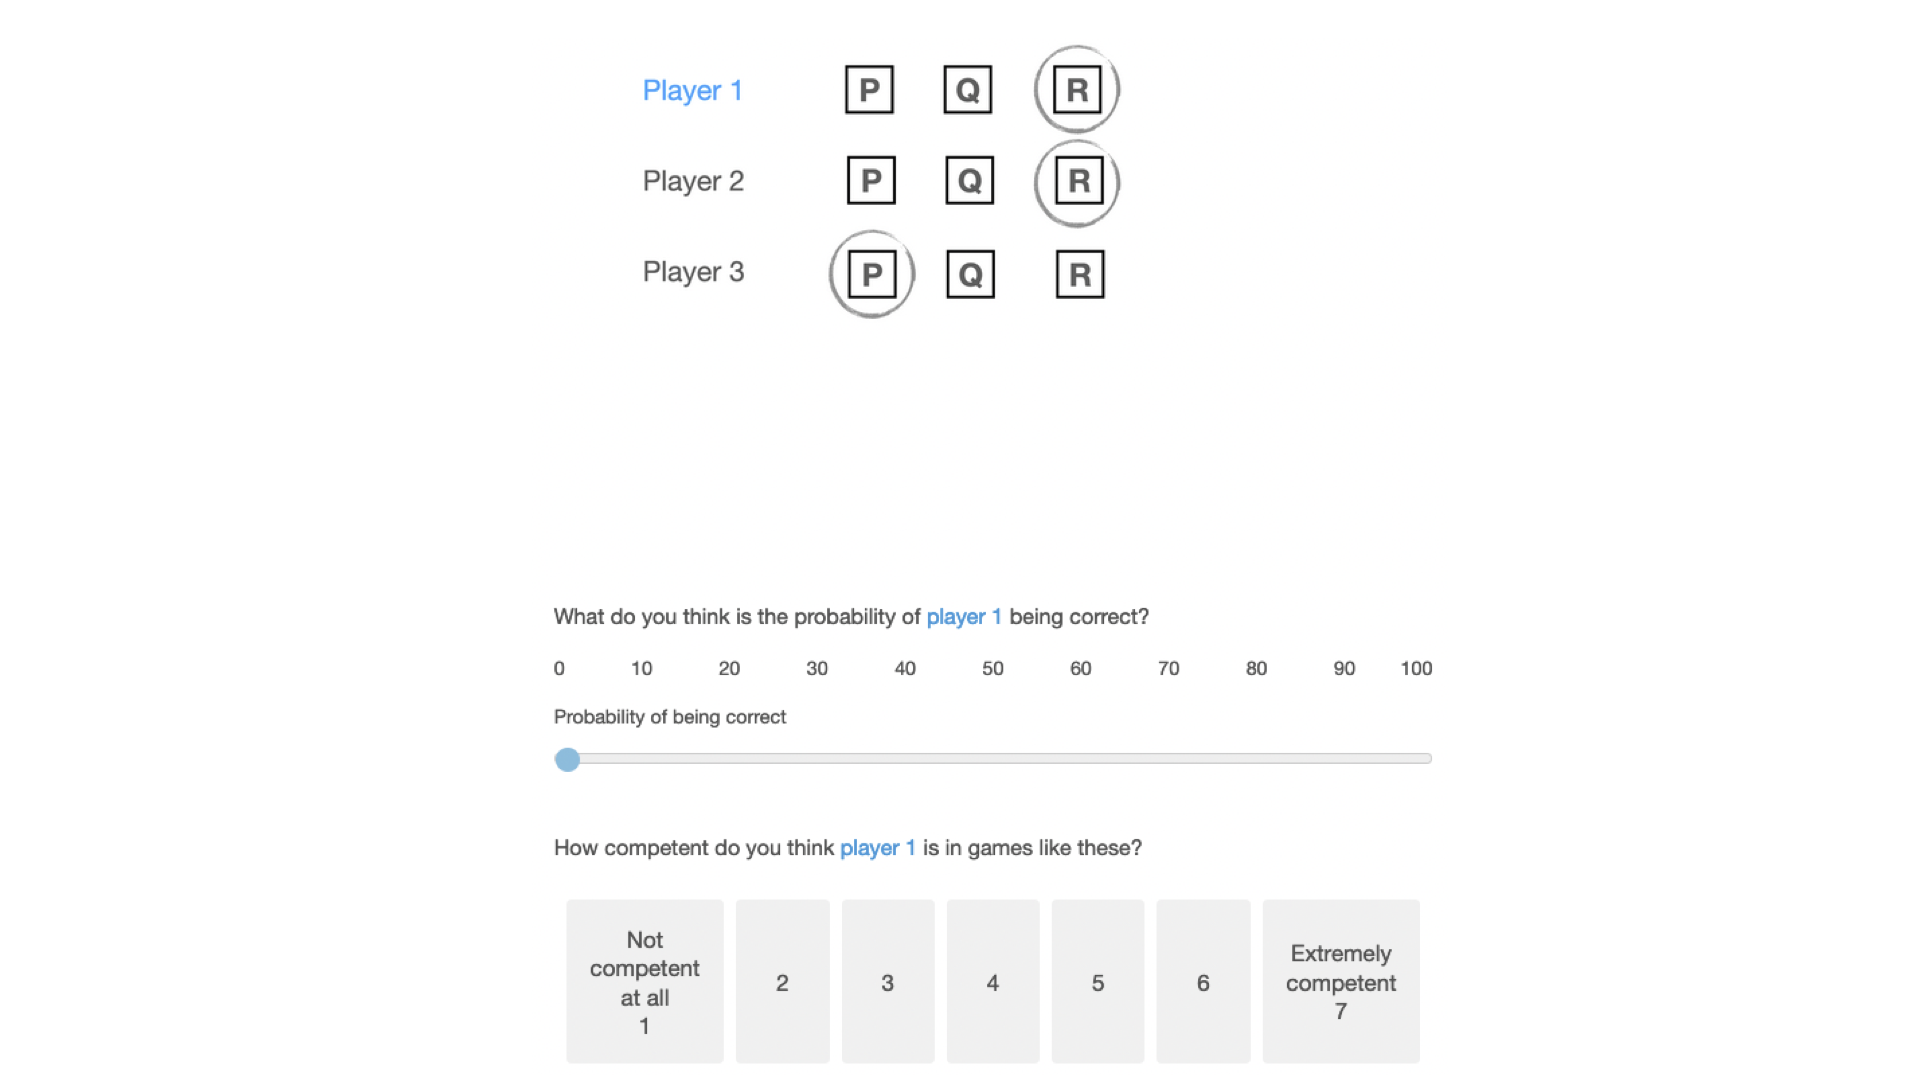
\includegraphics{figures/example_stimulus.png}
\caption{An example of a stimulus for the majority condition}
\end{figure}

\textbf{Convergence}. Convergence varies by the ratio of players
choosing the same response as the focal player (i.e.~the one that
participants evaluate). The levels of convergence are: (i) consensus,
where all three players pick the same option
{[}\texttt{coded\ value\ =\ 3}{]}; (ii) majority, where either the third
or second player picks the same option as the first player
{[}\texttt{coded\ value\ =\ 2}{]}; (iii) dissensus, where all three
players pick different options {[}\texttt{coded\ value\ =\ 1}{]}; (iv)
majority against the focal player's estimate, where the second and third
player pick the same option, but one that is different from the first
player's choice {[}\texttt{coded\ value\ =\ 0}{]}. In our analysis, we
treat convergence as a continuous variable, assigning the values in
squared parenthesis.

We manipulate convergence within participants. All participants see all
four conditions of convergence, with two stimuli (i.e.~game results) per
condition. Each participant therefore sees eight stimuli in total (4
convergence levels x 2 stimuli) .

\begin{longtable}[]{@{}
  >{\centering\arraybackslash}p{(\columnwidth - 4\tabcolsep) * \real{0.1704}}
  >{\centering\arraybackslash}p{(\columnwidth - 4\tabcolsep) * \real{0.4148}}
  >{\centering\arraybackslash}p{(\columnwidth - 4\tabcolsep) * \real{0.4148}}@{}}
\caption{Stimuli for 3 options condition by levels of
convergence}\tabularnewline
\toprule()
\begin{minipage}[b]{\linewidth}\centering
Level
\end{minipage} & \begin{minipage}[b]{\linewidth}\centering
Version a)
\end{minipage} & \begin{minipage}[b]{\linewidth}\centering
Version b)
\end{minipage} \\
\midrule()
\endfirsthead
\toprule()
\begin{minipage}[b]{\linewidth}\centering
Level
\end{minipage} & \begin{minipage}[b]{\linewidth}\centering
Version a)
\end{minipage} & \begin{minipage}[b]{\linewidth}\centering
Version b)
\end{minipage} \\
\midrule()
\endhead
opposing majority (0) &
\includegraphics[width=0.6\textwidth,height=\textheight]{figures/stimuli/opp_majority_3_a.png}
&
\includegraphics[width=0.6\textwidth,height=\textheight]{figures/stimuli/opp_majority_3_b.png} \\
dissensus (1) &
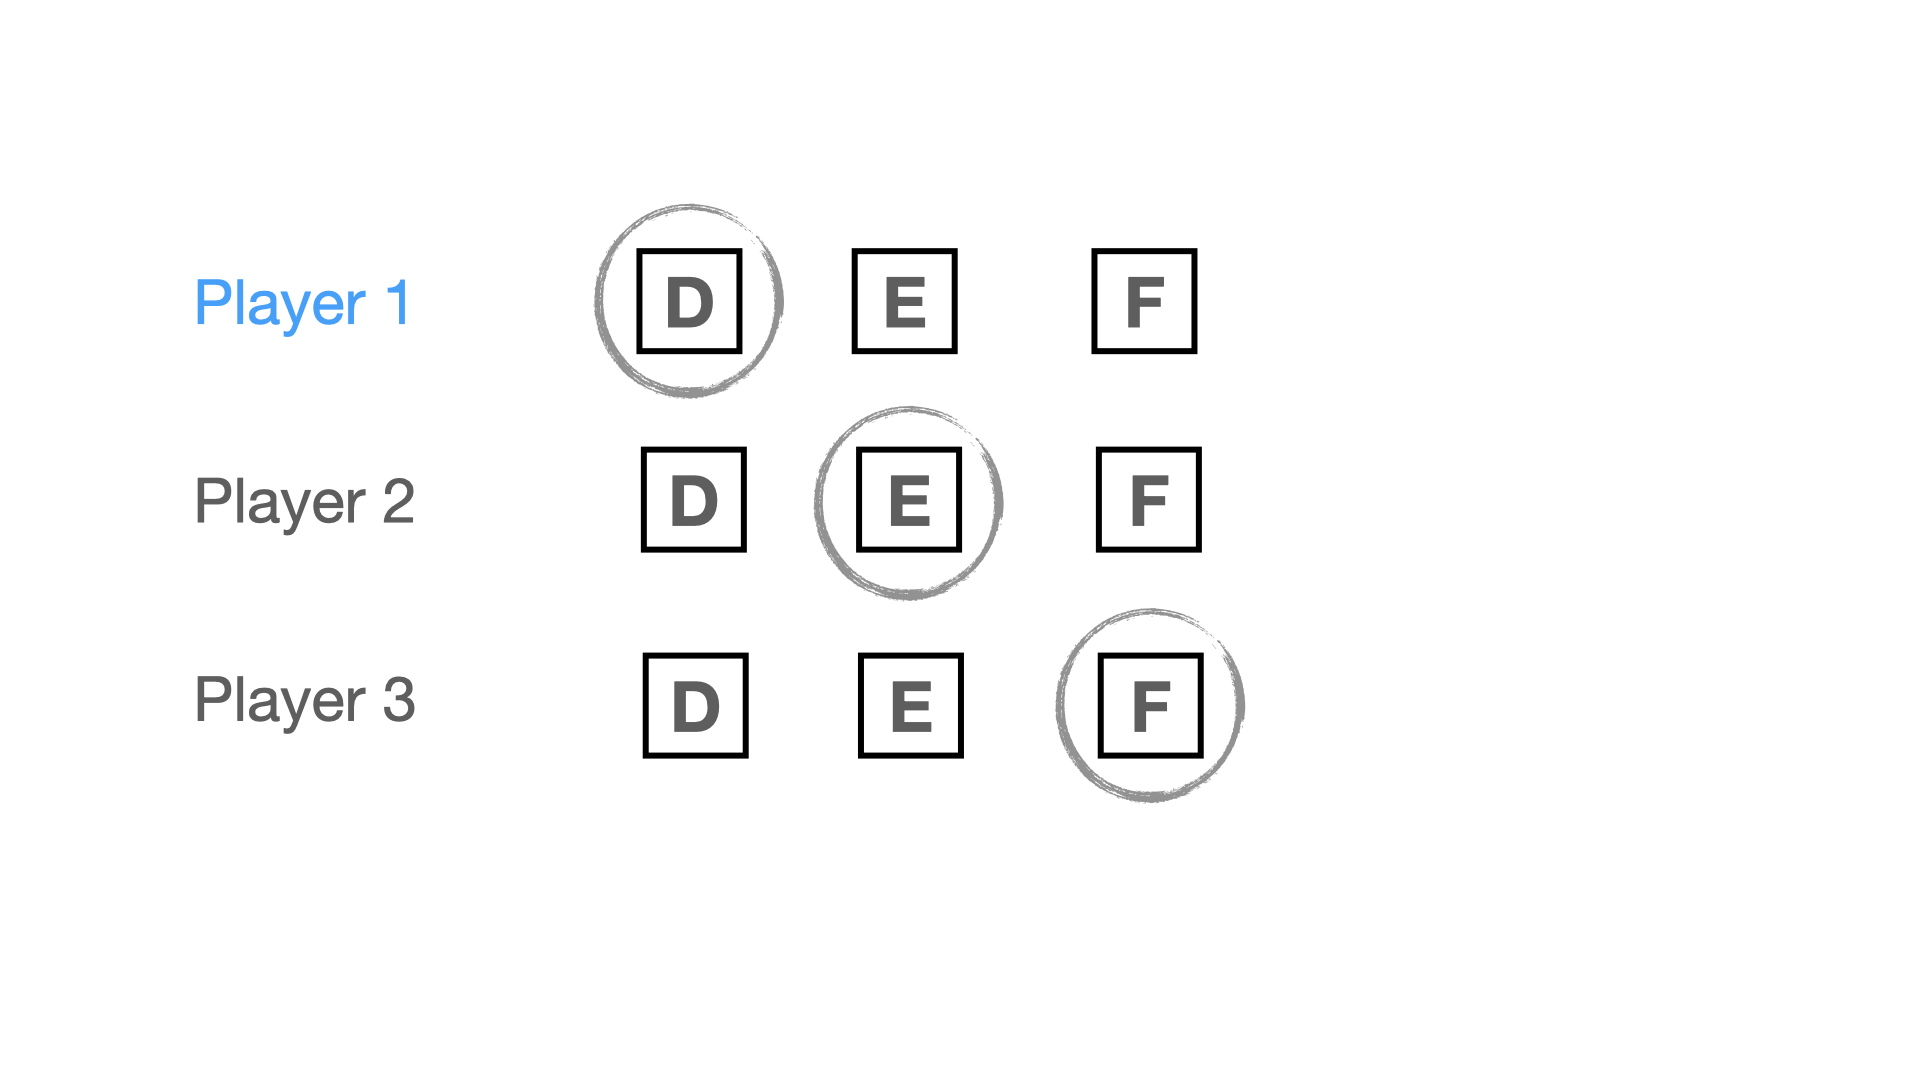
\includegraphics[width=0.6\textwidth,height=\textheight]{figures/stimuli/divergence_3_a.png}
&
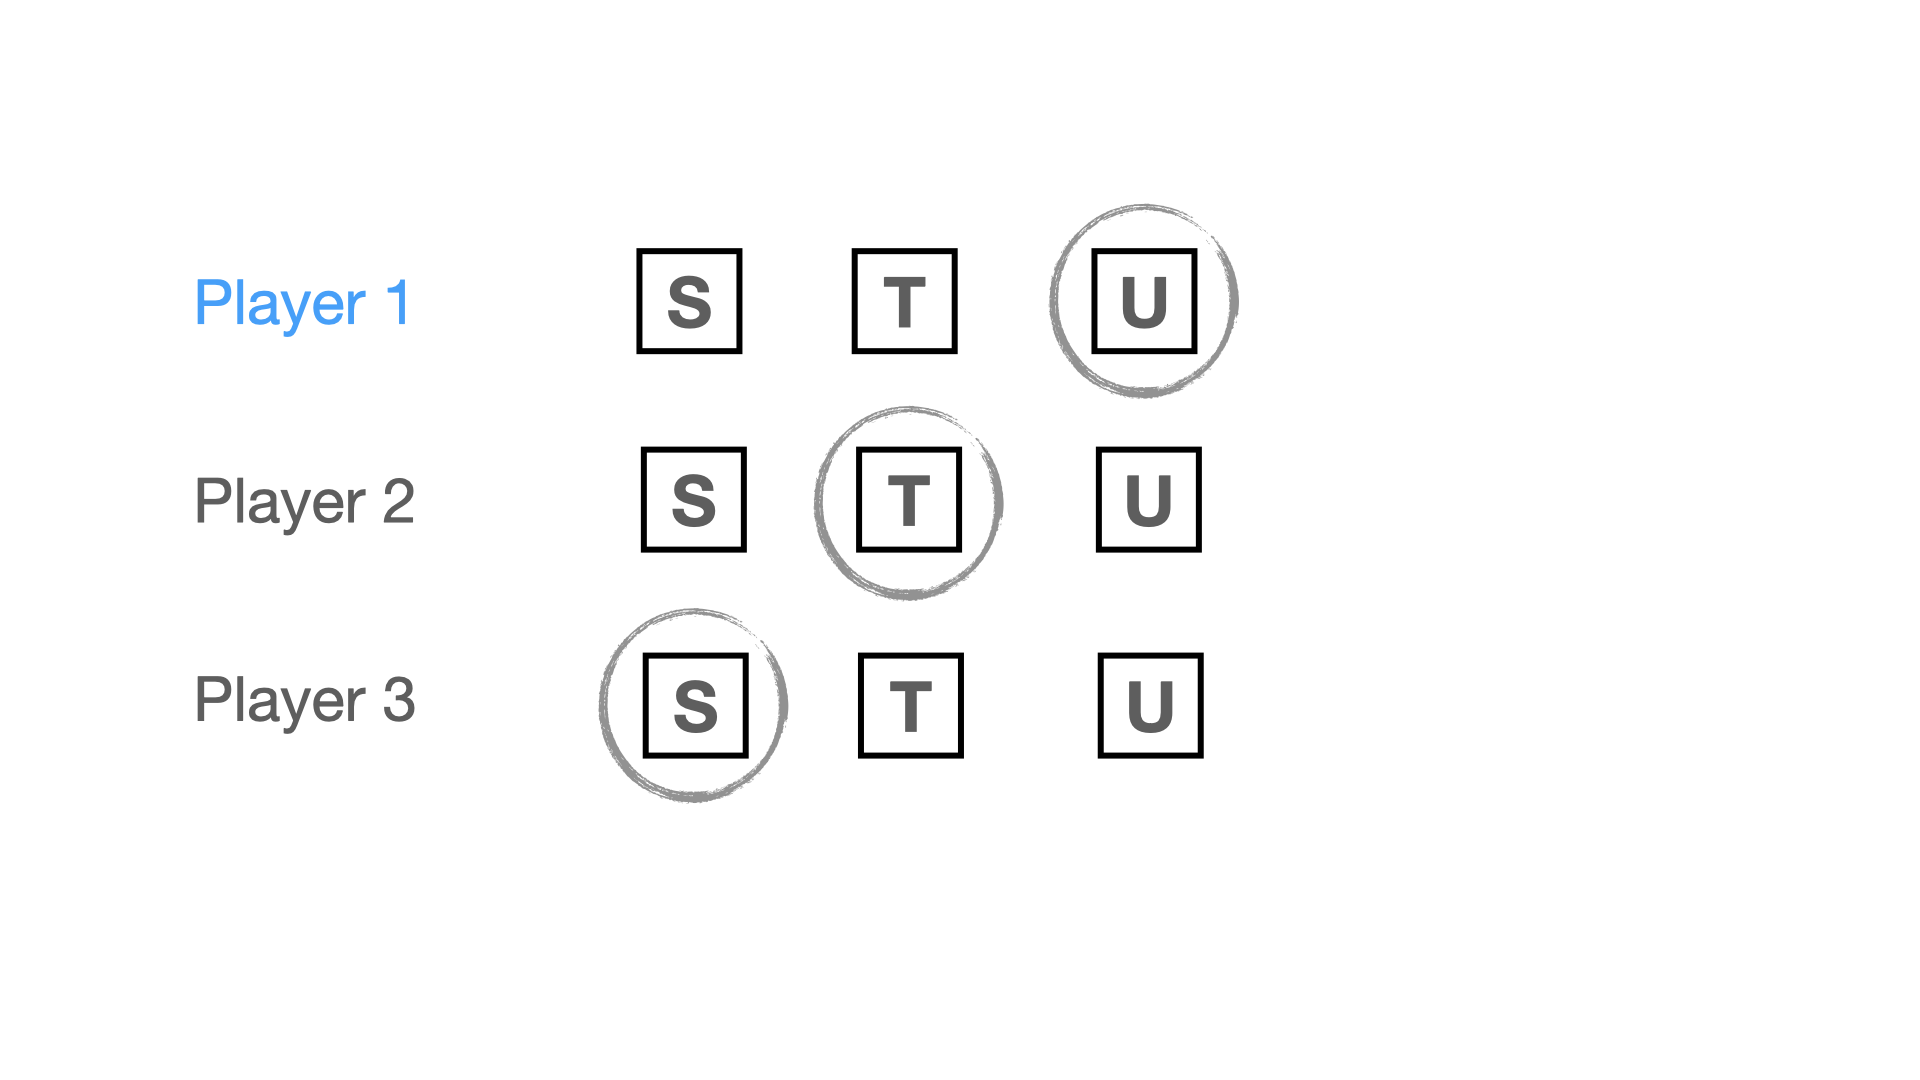
\includegraphics[width=0.6\textwidth,height=\textheight]{figures/stimuli/divergence_3_b.png} \\
majority (2) &
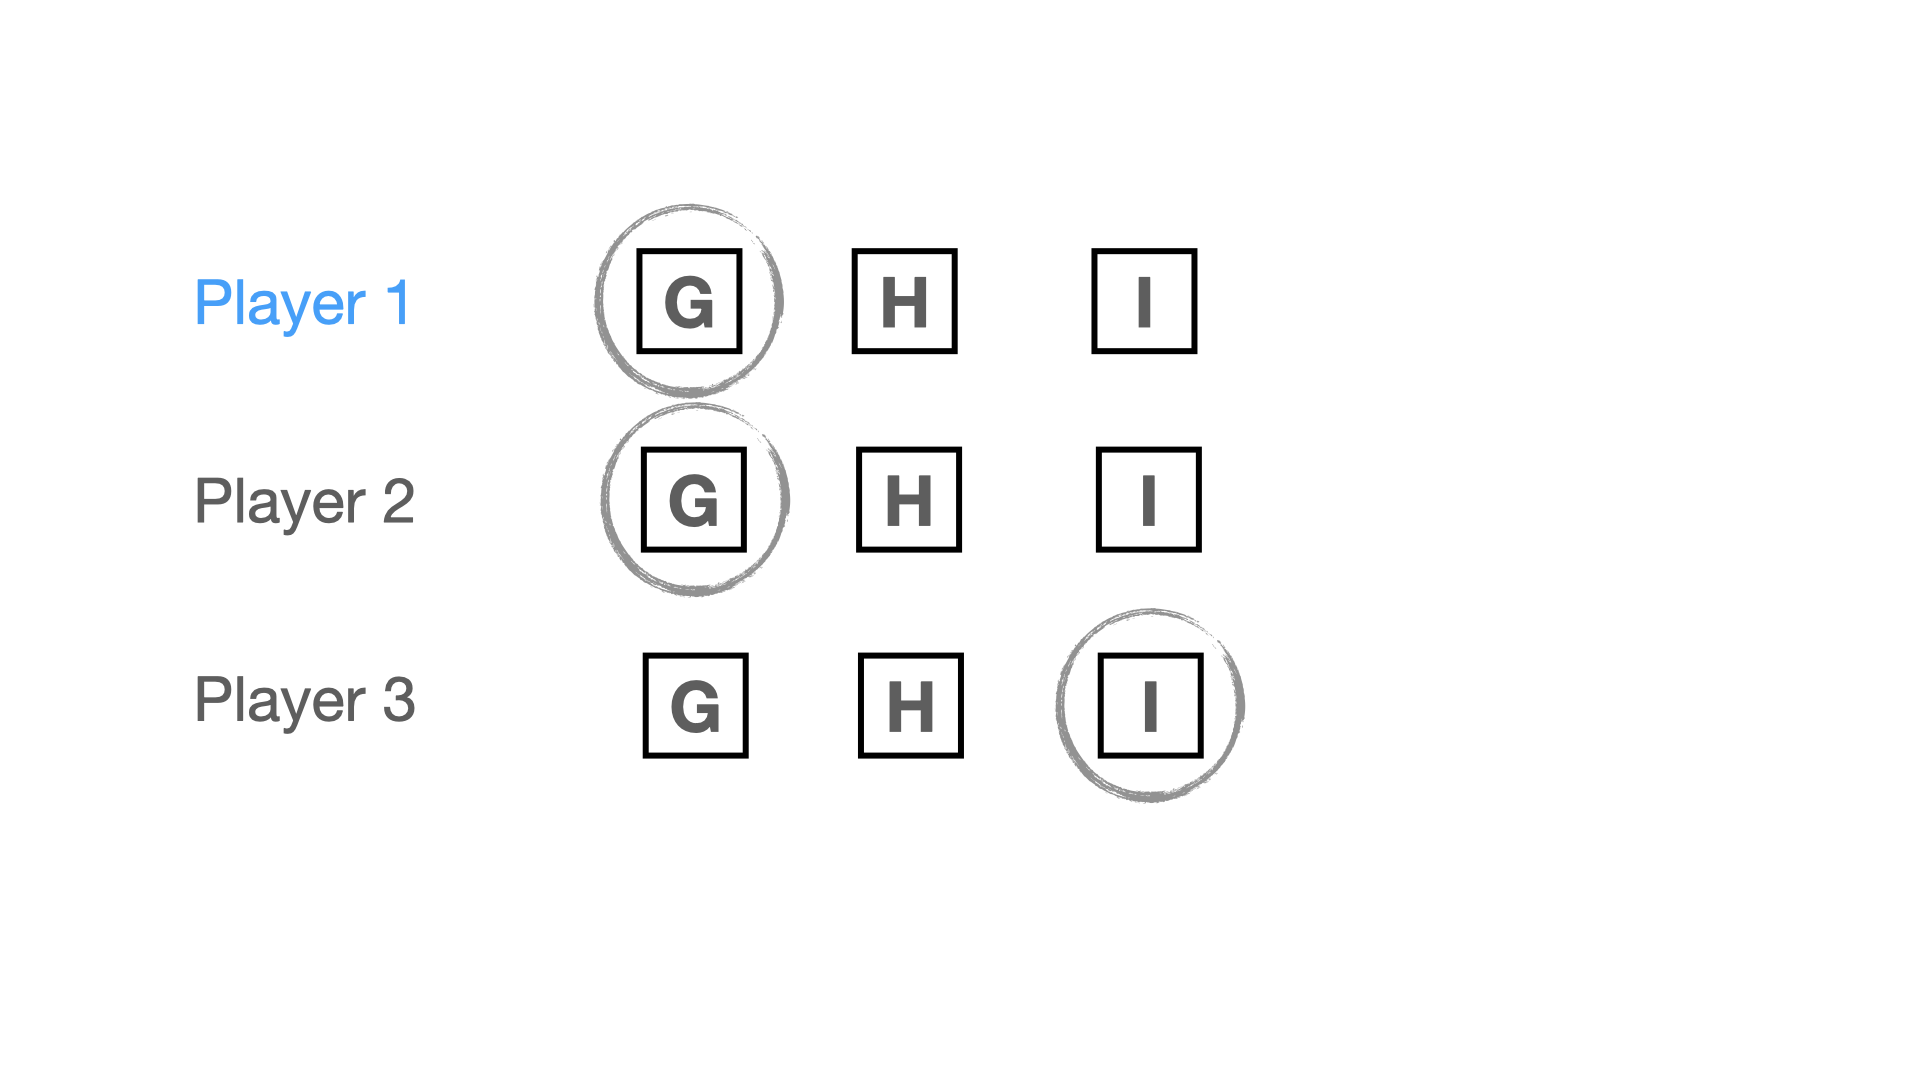
\includegraphics[width=0.6\textwidth,height=\textheight]{figures/stimuli/majority_3_a.png}
&
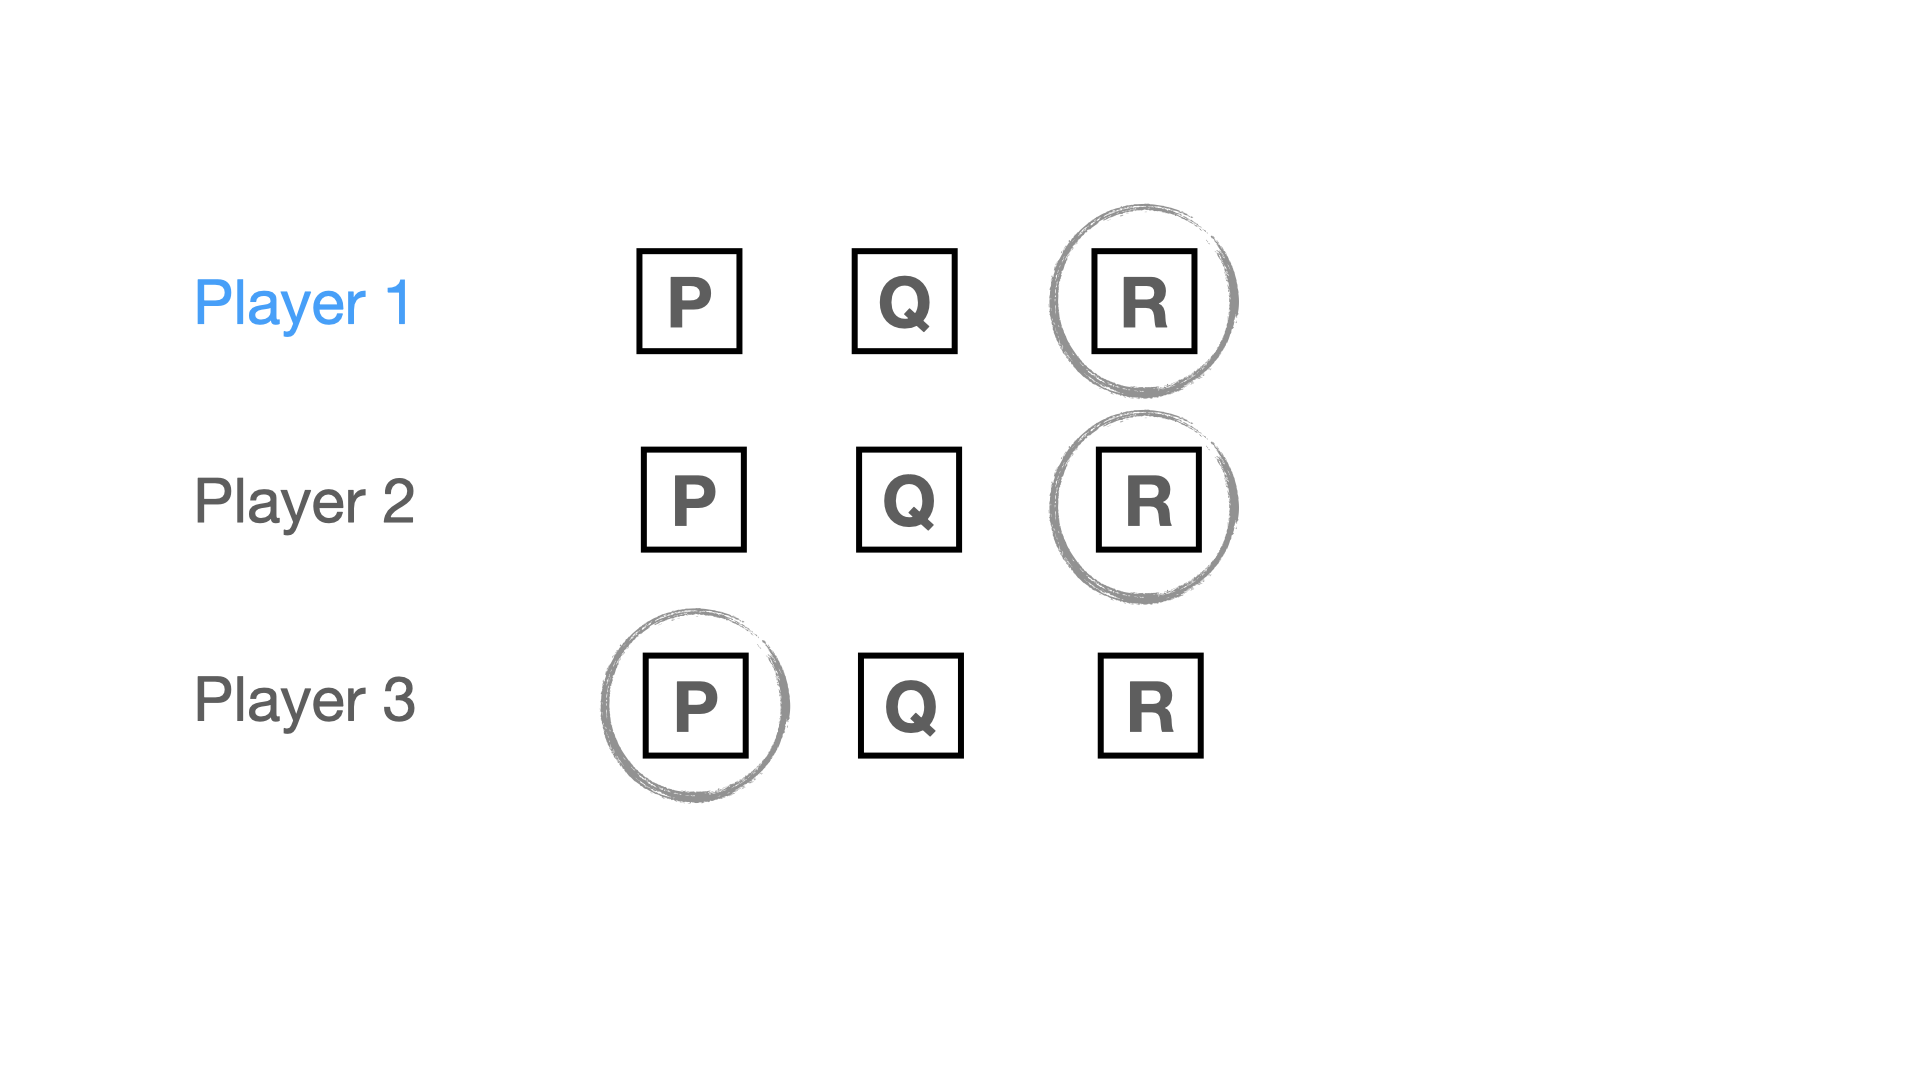
\includegraphics[width=0.6\textwidth,height=\textheight]{figures/stimuli/majority_3_b.png} \\
consensus (3) &
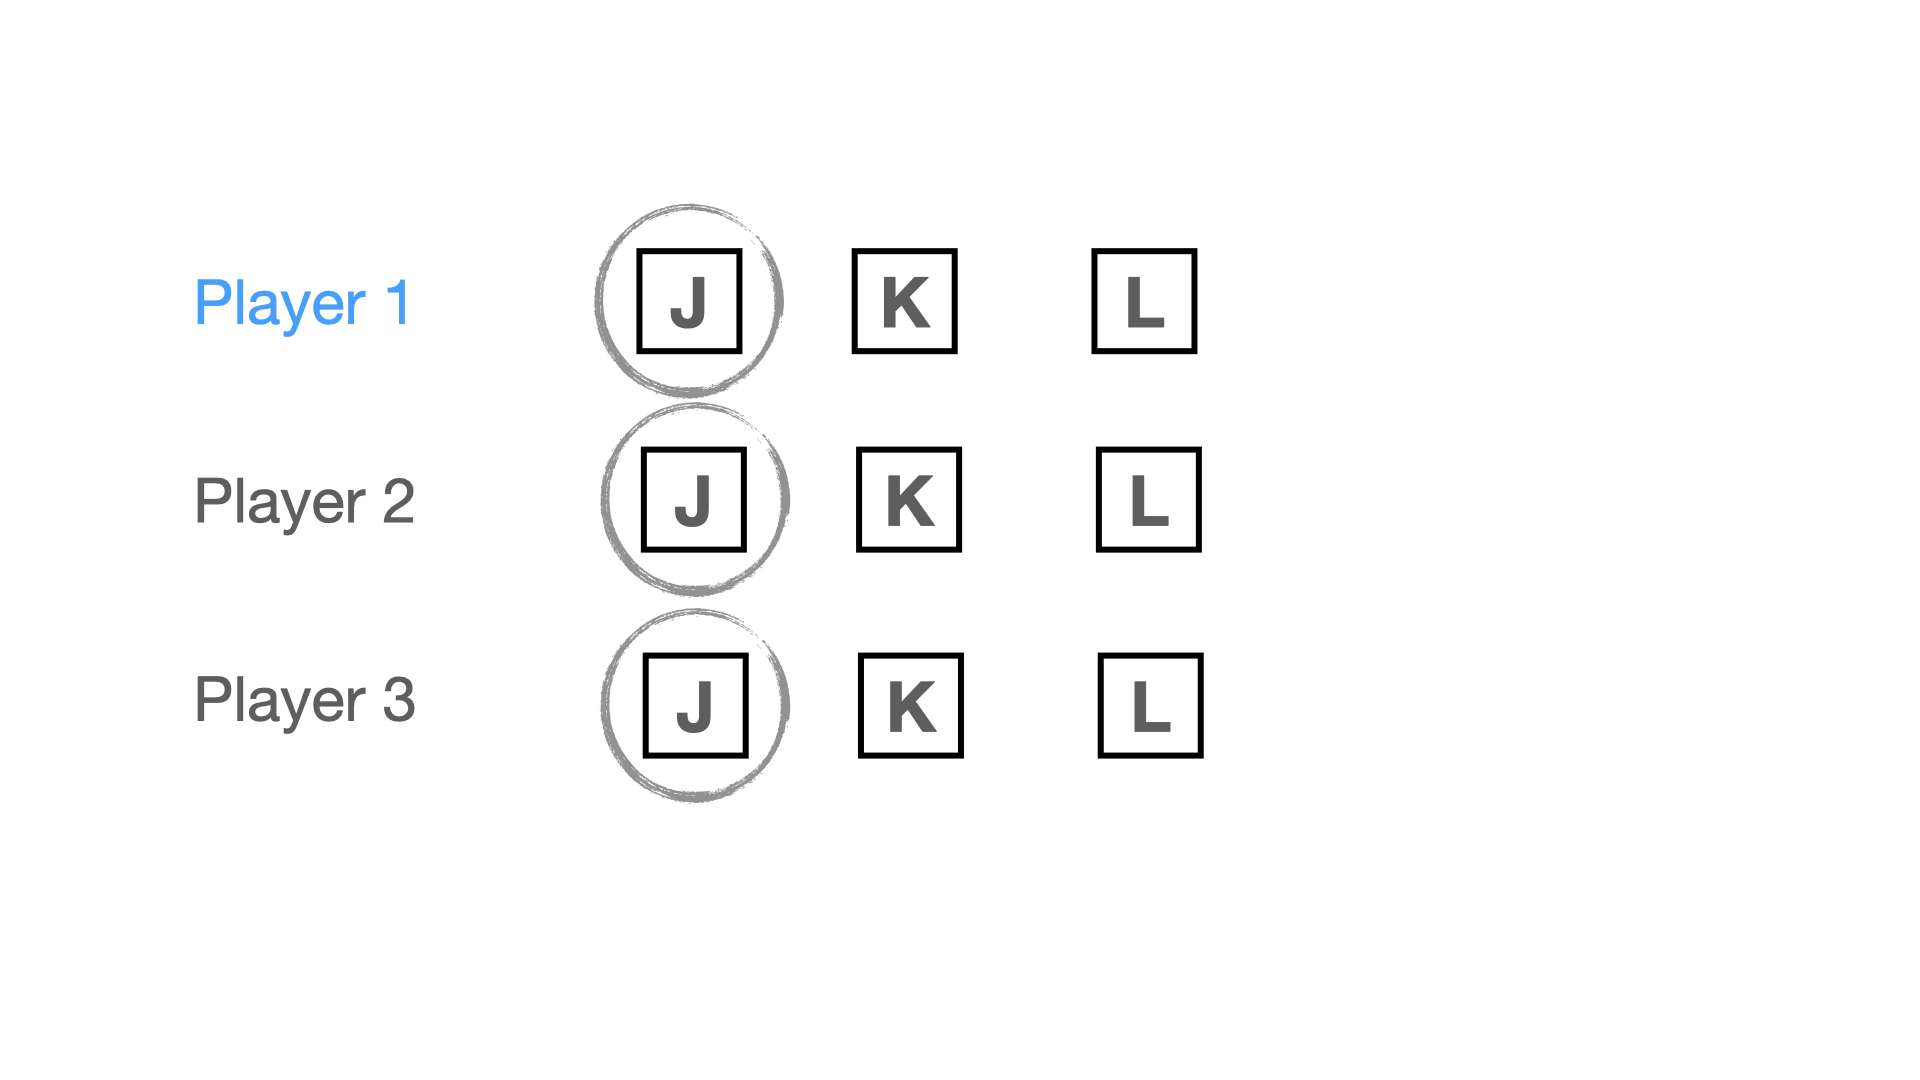
\includegraphics[width=0.6\textwidth,height=\textheight]{figures/stimuli/consensus_3_a.png}
&
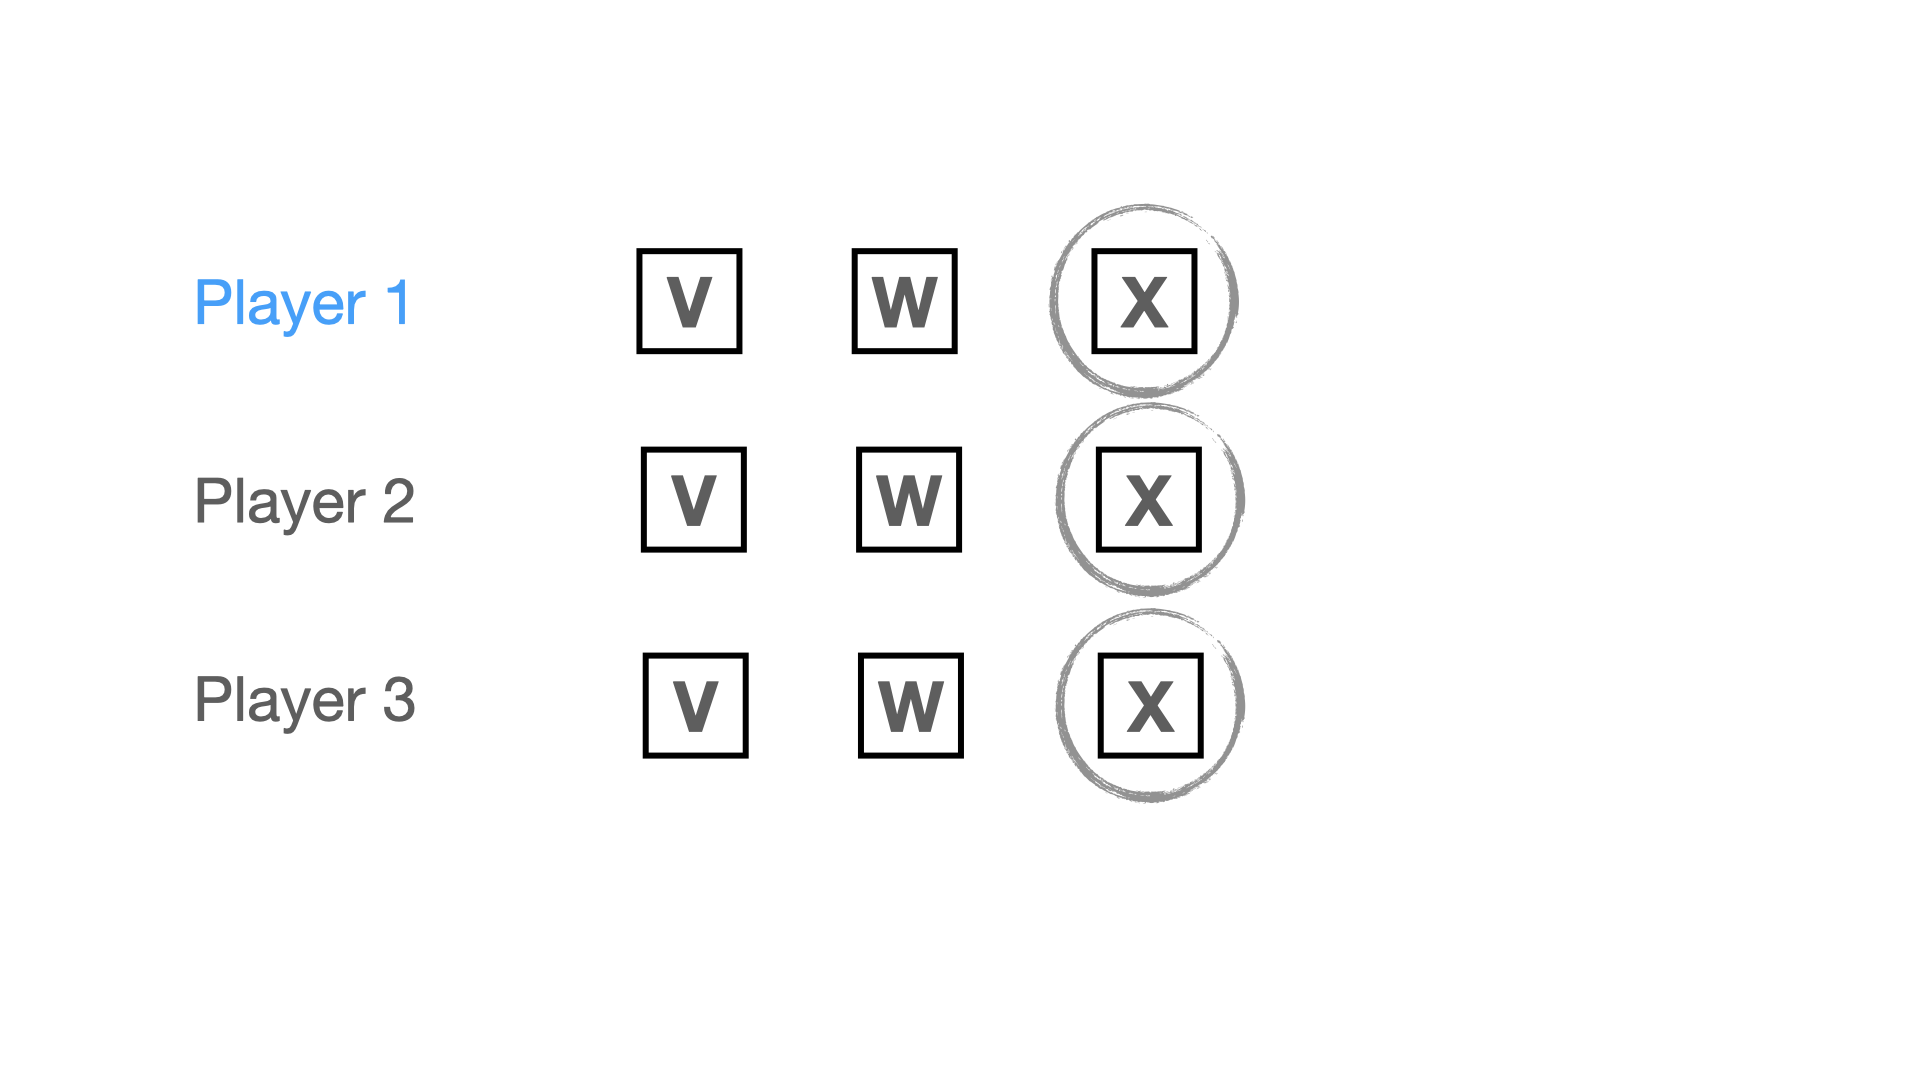
\includegraphics[width=0.6\textwidth,height=\textheight]{figures/stimuli/consensus_3_b.png} \\
\bottomrule()
\end{longtable}

\textbf{Options}. Independence has two levels: (i) `3' and (ii) `10'.

We manipulate independence between participants, i.e.~each participant
gets assigned to either the `3' or the `10' condition. All stimuli that
participants see in their respective condition will involve the same
number of choice options.

\begin{longtable}[]{@{}
  >{\centering\arraybackslash}p{(\columnwidth - 4\tabcolsep) * \real{0.1230}}
  >{\centering\arraybackslash}p{(\columnwidth - 4\tabcolsep) * \real{0.4344}}
  >{\centering\arraybackslash}p{(\columnwidth - 4\tabcolsep) * \real{0.4426}}@{}}
\caption{Example of a consensus stimulus for the two `Option'
conditions}\tabularnewline
\toprule()
\begin{minipage}[b]{\linewidth}\centering
Convergence
\end{minipage} & \begin{minipage}[b]{\linewidth}\centering
Options: 3
\end{minipage} & \begin{minipage}[b]{\linewidth}\centering
Options: 10
\end{minipage} \\
\midrule()
\endfirsthead
\toprule()
\begin{minipage}[b]{\linewidth}\centering
Convergence
\end{minipage} & \begin{minipage}[b]{\linewidth}\centering
Options: 3
\end{minipage} & \begin{minipage}[b]{\linewidth}\centering
Options: 10
\end{minipage} \\
\midrule()
\endhead
consensus (3) &
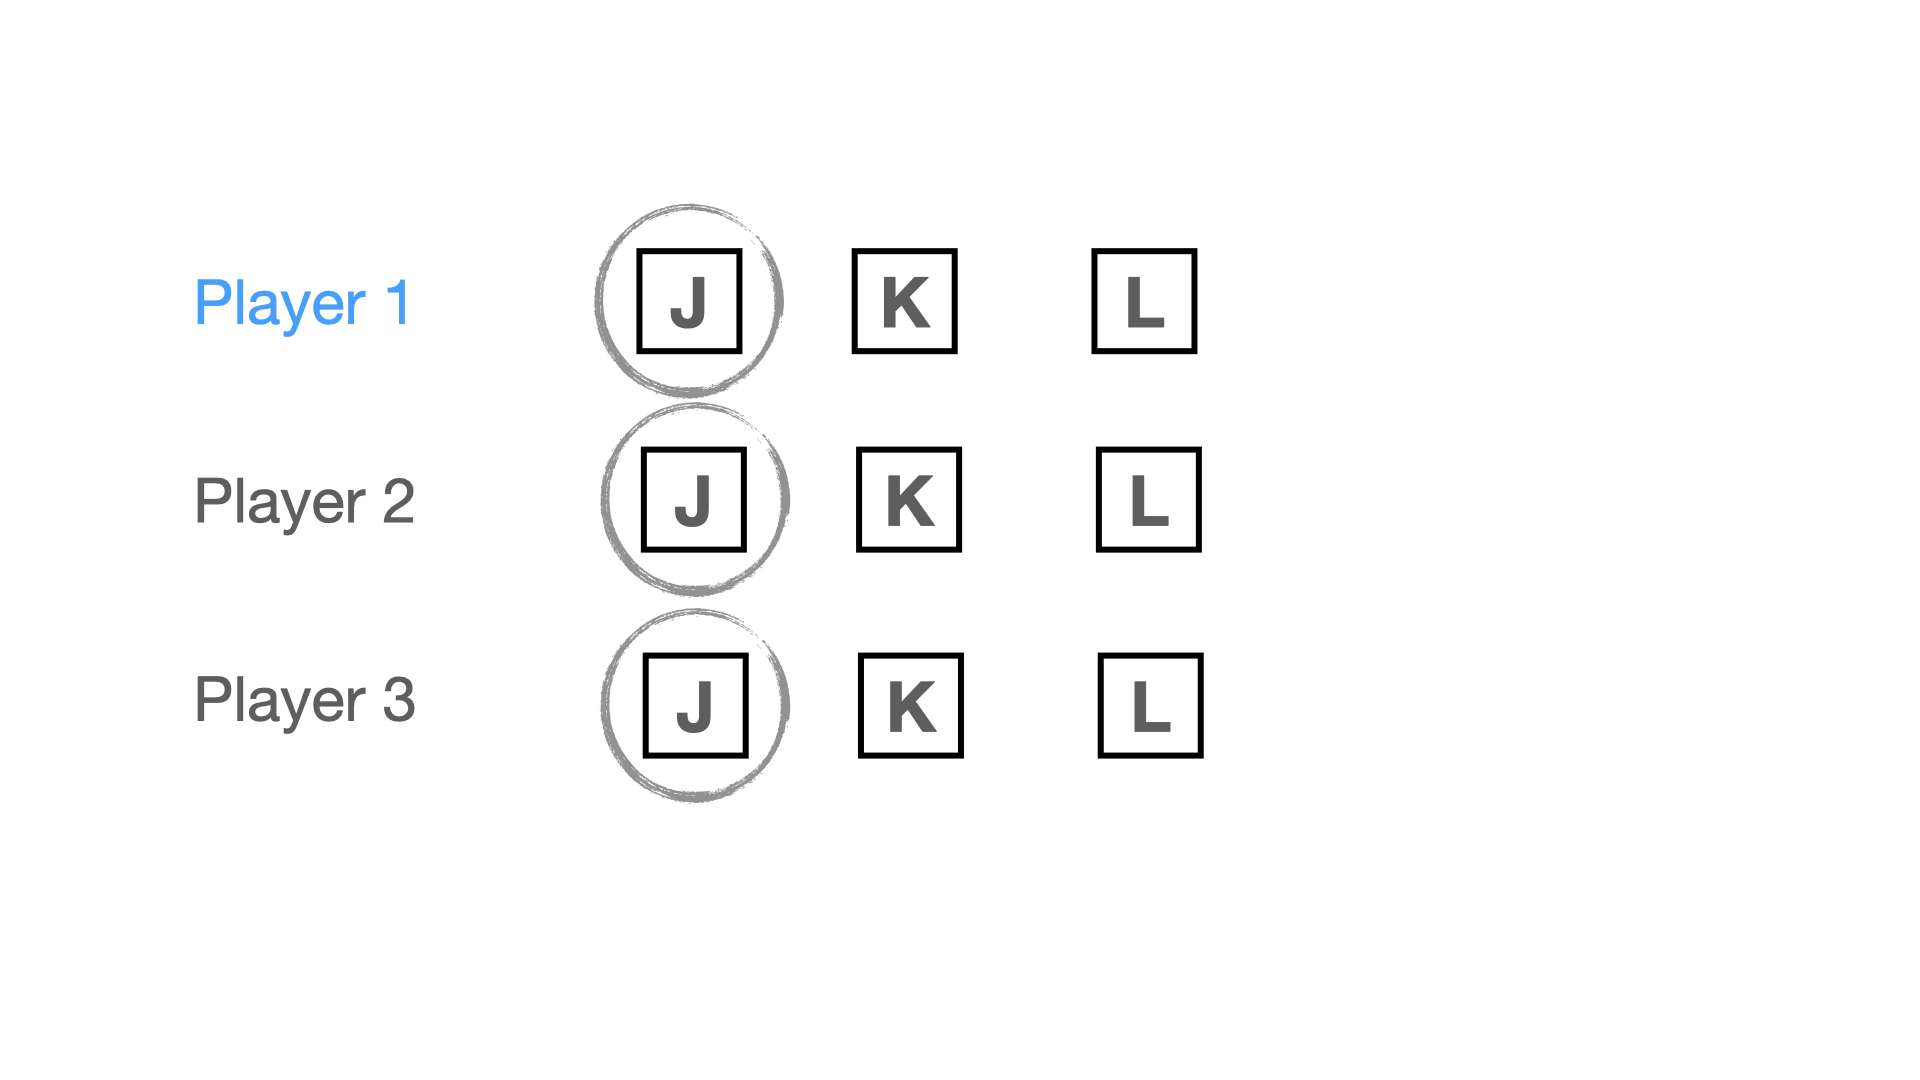
\includegraphics[width=0.6\textwidth,height=\textheight]{figures/stimuli/consensus_3_a.png}
&
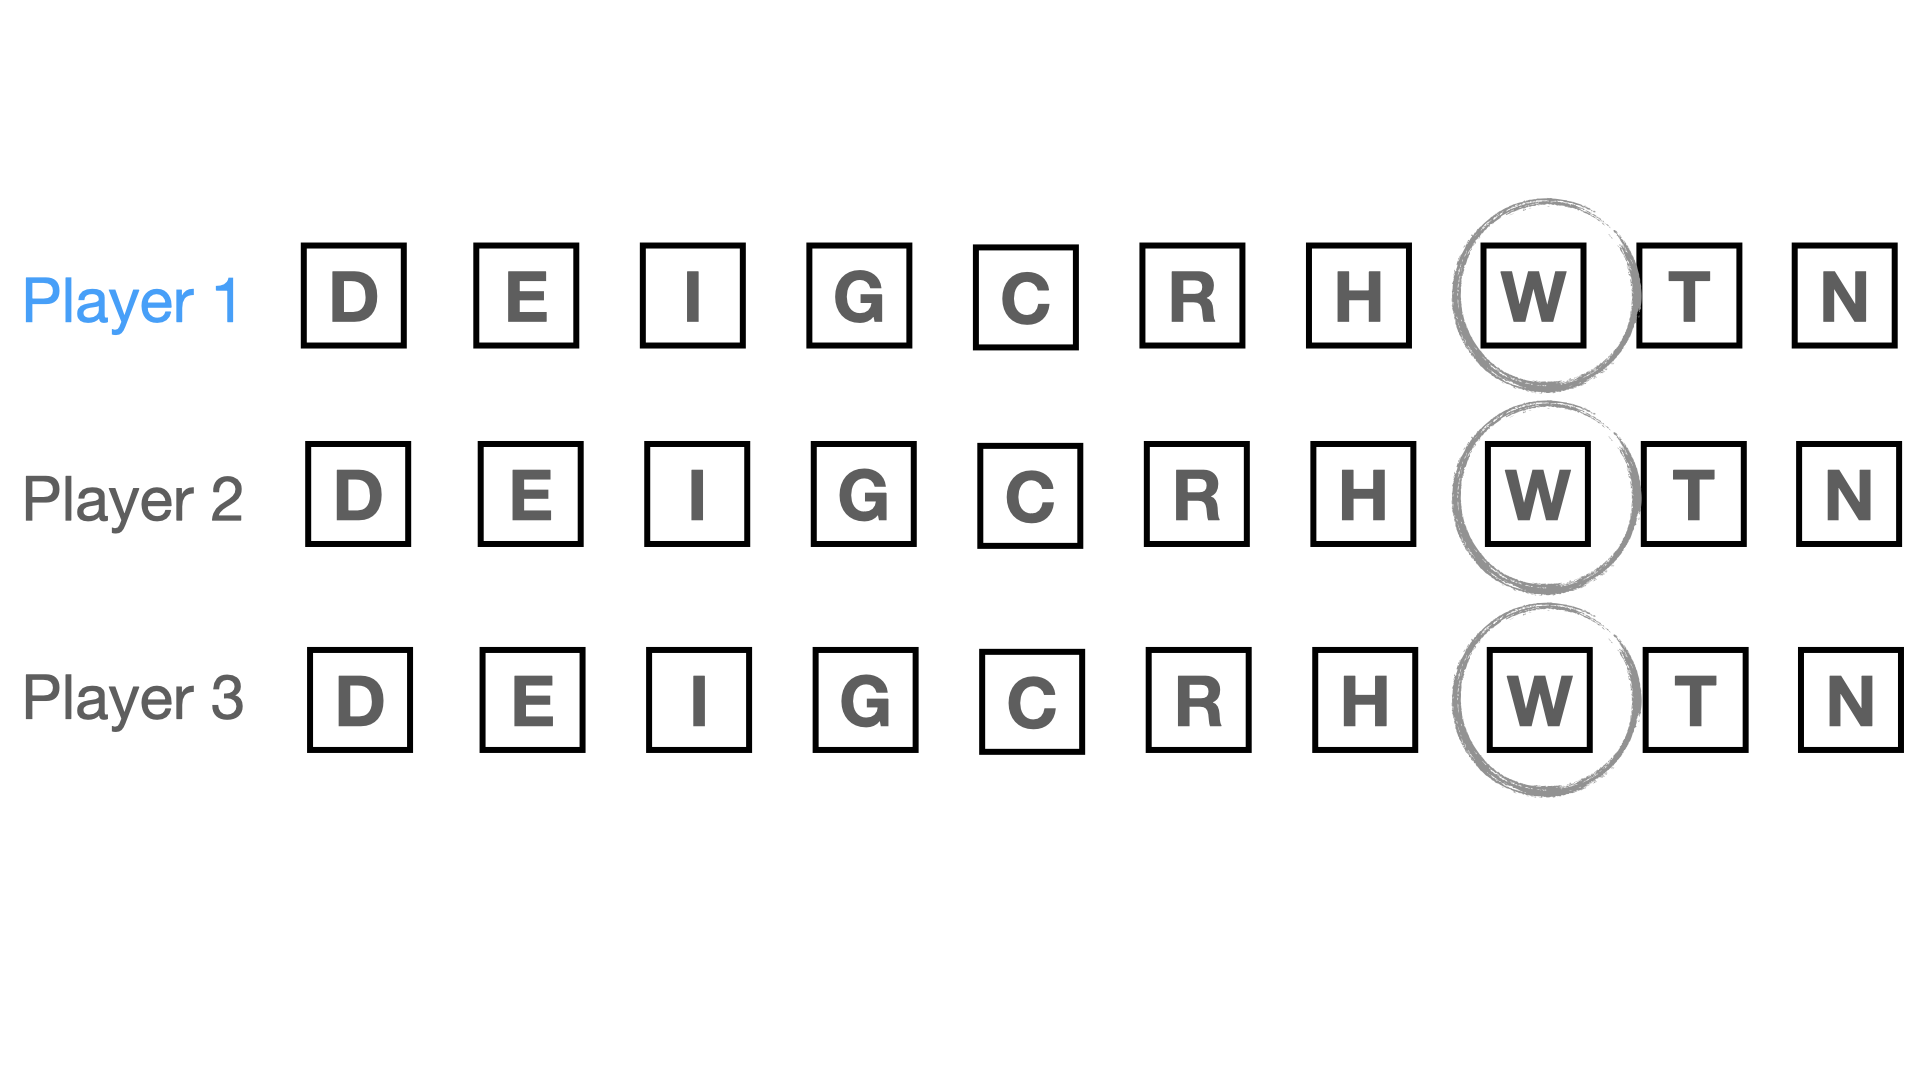
\includegraphics[width=0.6\textwidth,height=\textheight]{figures/stimuli/consensus_10_a.png} \\
\bottomrule()
\end{longtable}

As outcome variables, we will measure people's perceived accuracy and
competence of player one.

\textbf{Accuracy}. We ask participants ``What do you think is the
probability of player 1 being correct?''. Participants answer with a
slider from 0 to 100.

\textbf{Competence}. We ask participants ``How competent do you think
player 1 is in games like these?'' Participants answer on a 7-point
Likert scale (from ``not competent at all'' to ``extremely competent'').

\hypertarget{iv.-hypotheses}{%
\section{IV. Hypotheses}\label{iv.-hypotheses}}

Considering only \texttt{3} options condition of the experiment at hand,
we expect the findings of experiment four to replicate. In experiment
four, players would choose among \texttt{3} options.

\hypertarget{h1a-participants-perceive-an-estimate-of-an-independent-informant-as-more-accurate-the-more-it-converges-with-the-estimates-of-other-informants-given-three-choice-options.}{%
\subsubsection{H1a: Participants perceive an estimate of an independent
informant as more accurate the more it converges with the estimates of
other informants, given three choice
options.}\label{h1a-participants-perceive-an-estimate-of-an-independent-informant-as-more-accurate-the-more-it-converges-with-the-estimates-of-other-informants-given-three-choice-options.}}

To test this hypothesis, we only consider participants assigned to the
\texttt{3} options condition.

We use a linear mixed effect model with random intercept and random
slope per participant. Should this model yield convergence issues, we
will use a model with random intercept only.

In all our models we treat \texttt{convergence} as a continuous
variable. We will, however, include robustness checks where we treat
convergence as a categorical variable, allowing to inspect difference
between different levels.

\begin{Shaded}
\begin{Highlighting}[]
\CommentTok{\# models for accuracy}

\CommentTok{\# random intercept and slope by participants}
\NormalTok{model\_accuracy }\OtherTok{\textless{}{-}} \FunctionTok{lmer}\NormalTok{(accuracy }\SpecialCharTok{\textasciitilde{}}\NormalTok{ convergence }\SpecialCharTok{+}\NormalTok{ (}\DecValTok{1} \SpecialCharTok{+}\NormalTok{ convergence }\SpecialCharTok{|}\NormalTok{ id), }
                       \AttributeTok{data =}\NormalTok{ data }\SpecialCharTok{\%\textgreater{}\%} \FunctionTok{filter}\NormalTok{(options }\SpecialCharTok{==} \StringTok{"3"}\NormalTok{))}

\CommentTok{\# in case of non{-}convergence: random intercept by participants only}
\NormalTok{alt\_model\_accuracy }\OtherTok{\textless{}{-}} \FunctionTok{lmer}\NormalTok{(accuracy }\SpecialCharTok{\textasciitilde{}}\NormalTok{ convergence }\SpecialCharTok{+}\NormalTok{ (}\DecValTok{1} \SpecialCharTok{|}\NormalTok{ id), }
                           \AttributeTok{data =}\NormalTok{ data }\SpecialCharTok{\%\textgreater{}\%} \FunctionTok{filter}\NormalTok{(options }\SpecialCharTok{==} \StringTok{"3"}\NormalTok{))}
\end{Highlighting}
\end{Shaded}

\hypertarget{h1b-participants-perceive-an-independent-informant-as-more-competent-the-more-their-estimate-converges-with-the-estimates-of-other-informants-given-three-choice-options.}{%
\subsubsection{H1b: Participants perceive an independent informant as
more competent the more their estimate converges with the estimates of
other informants, given three choice
options.}\label{h1b-participants-perceive-an-independent-informant-as-more-competent-the-more-their-estimate-converges-with-the-estimates-of-other-informants-given-three-choice-options.}}

To test this hypothesis, we only consider participants assigned to the
\texttt{3} options condition.

We will proceed in the same way for \texttt{competence} as we did for
\texttt{accuracy} above.

\begin{Shaded}
\begin{Highlighting}[]
\CommentTok{\# models for competence}

\CommentTok{\# random intercept and slope by participants}
\NormalTok{model\_competence }\OtherTok{\textless{}{-}} \FunctionTok{lmer}\NormalTok{(competence }\SpecialCharTok{\textasciitilde{}}\NormalTok{ convergence }\SpecialCharTok{+} 
\NormalTok{                           (}\DecValTok{1} \SpecialCharTok{+}\NormalTok{ convergence }\SpecialCharTok{|}\NormalTok{ id), }
                         \AttributeTok{data =}\NormalTok{ data }\SpecialCharTok{\%\textgreater{}\%} \FunctionTok{filter}\NormalTok{(options }\SpecialCharTok{==} \StringTok{"3"}\NormalTok{))}

\CommentTok{\# in case of non{-}convergence: random intercept by participants only}
\NormalTok{alt\_model\_competence }\OtherTok{\textless{}{-}} \FunctionTok{lmer}\NormalTok{(competence }\SpecialCharTok{\textasciitilde{}}\NormalTok{ convergence }\SpecialCharTok{+}\NormalTok{ (}\DecValTok{1} \SpecialCharTok{|}\NormalTok{ id), }
                             \AttributeTok{data =}\NormalTok{ data }\SpecialCharTok{\%\textgreater{}\%} \FunctionTok{filter}\NormalTok{(options }\SpecialCharTok{==} \StringTok{"3"}\NormalTok{))}
\end{Highlighting}
\end{Shaded}

How about a context in which informants (i.e.~the fictive players) could
choose not among 3, but among 10 options? In line with our findings from
experiment three, we predict that effects of convergence are more
positive when there are more choice options:

\hypertarget{h2a-the-effect-of-convergence-on-accuracy-h1a-is-more-positive-in-a-context-where-informants-can-choose-among-ten-response-options-compared-to-when-they-can-choose-among-only-three.}{%
\subsubsection{H2a: The effect of convergence on accuracy (H1a) is more
positive in a context where informants can choose among ten response
options compared to when they can choose among only
three.}\label{h2a-the-effect-of-convergence-on-accuracy-h1a-is-more-positive-in-a-context-where-informants-can-choose-among-ten-response-options-compared-to-when-they-can-choose-among-only-three.}}

To test this hypothesis, we consider the full data.

The resulting estimate of the interaction term will provide the test for
our hypothesis.

\begin{Shaded}
\begin{Highlighting}[]
\CommentTok{\# models for accuracy}

\CommentTok{\# random intercept and slope by participants}
\NormalTok{model\_accuracy }\OtherTok{\textless{}{-}} \FunctionTok{lmer}\NormalTok{(accuracy }\SpecialCharTok{\textasciitilde{}}\NormalTok{ convergence }\SpecialCharTok{+}\NormalTok{ options }\SpecialCharTok{+} 
\NormalTok{                            options}\SpecialCharTok{*}\NormalTok{convergence }\SpecialCharTok{+}\NormalTok{ (}\DecValTok{1} \SpecialCharTok{+}\NormalTok{ convergence }\SpecialCharTok{|}\NormalTok{ id), }
                       \AttributeTok{data =}\NormalTok{ data)}

\CommentTok{\# in case of non{-}convergence: random intercept by participants only}
\NormalTok{alt\_model\_accuracy }\OtherTok{\textless{}{-}} \FunctionTok{lmer}\NormalTok{(accuracy }\SpecialCharTok{\textasciitilde{}}\NormalTok{ convergence }\SpecialCharTok{+}\NormalTok{ options }\SpecialCharTok{+} 
\NormalTok{                            options}\SpecialCharTok{*}\NormalTok{convergence }\SpecialCharTok{+}\NormalTok{ (}\DecValTok{1} \SpecialCharTok{|}\NormalTok{ id), }
                           \AttributeTok{data =}\NormalTok{ data)}
\end{Highlighting}
\end{Shaded}

\hypertarget{h2b-the-effect-of-convergence-on-competence-h1b-is-more-positive-in-a-context-where-informants-can-choose-among-ten-response-options-compared-to-when-they-can-choose-among-only-three.}{%
\subsubsection{H2b: The effect of convergence on competence (H1b) is
more positive in a context where informants can choose among ten
response options compared to when they can choose among only
three.}\label{h2b-the-effect-of-convergence-on-competence-h1b-is-more-positive-in-a-context-where-informants-can-choose-among-ten-response-options-compared-to-when-they-can-choose-among-only-three.}}

To test this hypothesis, we consider the full data.

The resulting estimate of the interaction term will provide the test for
our hypothesis.

\begin{Shaded}
\begin{Highlighting}[]
\CommentTok{\# models for competence}

\CommentTok{\# random intercept and slope by participants}
\NormalTok{model\_competence }\OtherTok{\textless{}{-}} \FunctionTok{lmer}\NormalTok{(competence }\SpecialCharTok{\textasciitilde{}}\NormalTok{ convergence }\SpecialCharTok{+}\NormalTok{ options }\SpecialCharTok{+} 
\NormalTok{                            options}\SpecialCharTok{*}\NormalTok{convergence }\SpecialCharTok{+}\NormalTok{ (}\DecValTok{1} \SpecialCharTok{+}\NormalTok{ convergence }\SpecialCharTok{|}\NormalTok{ id), }
                       \AttributeTok{data =}\NormalTok{ data)}

\CommentTok{\# in case of non{-}convergence: random intercept by participants only}
\NormalTok{alt\_model\_competence }\OtherTok{\textless{}{-}} \FunctionTok{lmer}\NormalTok{(competence }\SpecialCharTok{\textasciitilde{}}\NormalTok{ convergence }\SpecialCharTok{+}\NormalTok{ options }\SpecialCharTok{+} 
\NormalTok{                            options}\SpecialCharTok{*}\NormalTok{convergence }\SpecialCharTok{+}\NormalTok{ (}\DecValTok{1} \SpecialCharTok{|}\NormalTok{ id), }
                           \AttributeTok{data =}\NormalTok{ data)}
\end{Highlighting}
\end{Shaded}

\hypertarget{robustness-checks}{%
\section{Robustness checks}\label{robustness-checks}}

\hypertarget{convergence-as-categorical-variable}{%
\subsection{Convergence as categorical
variable}\label{convergence-as-categorical-variable}}

In the models above, we treated convergence as a continuous variable.
Based on the different levels, we will build a categorical variable,
\texttt{convergence\_categorical}.

\begin{Shaded}
\begin{Highlighting}[]
\CommentTok{\# make a categorical variable from \textasciigrave{}convergence\textasciigrave{}}
\NormalTok{data }\OtherTok{\textless{}{-}}\NormalTok{ data }\SpecialCharTok{\%\textgreater{}\%} 
  \FunctionTok{mutate}\NormalTok{(}\AttributeTok{convergence\_categorical =} \FunctionTok{recode\_factor}\NormalTok{(convergence, }
                                                 \StringTok{\textasciigrave{}}\AttributeTok{0}\StringTok{\textasciigrave{}} \OtherTok{=} \StringTok{"opposing majority"}\NormalTok{, }
                                                 \StringTok{\textasciigrave{}}\AttributeTok{1}\StringTok{\textasciigrave{}} \OtherTok{=} \StringTok{"divergence"}\NormalTok{, }
                                                 \StringTok{\textasciigrave{}}\AttributeTok{2}\StringTok{\textasciigrave{}} \OtherTok{=} \StringTok{"majority"}\NormalTok{, }
                                                 \StringTok{\textasciigrave{}}\AttributeTok{3}\StringTok{\textasciigrave{}} \OtherTok{=} \StringTok{"consensus"}\NormalTok{,}
                                                 \AttributeTok{.default =} \ConstantTok{NA\_character\_}\NormalTok{)}
\NormalTok{         )}

\FunctionTok{levels}\NormalTok{(data}\SpecialCharTok{$}\NormalTok{convergence\_categorical)}
\end{Highlighting}
\end{Shaded}

\begin{verbatim}
## [1] "opposing majority" "divergence"        "majority"         
## [4] "consensus"
\end{verbatim}

We run the same models outlined in the hypotheses section, but replacing
\texttt{convergence} with \texttt{convergence\_categorical}. This also
allows us to inspect heterogeneity in differences between levels (with
respect to the baseline, i.e.~``opposing majority'').

\hypertarget{alternative-stimuli-with-greater-distance}{%
\subsection{Alternative stimuli with greater
distance}\label{alternative-stimuli-with-greater-distance}}

Pick an example stimulus as earlier for illustrating choice options. See
all stimuli in appendix.

\hypertarget{exclusions}{%
\section{Exclusions}\label{exclusions}}

We will exclude participants failing (i.e.~participants not answering
the question or writing anything that does not at least resemble ``I pay
attention'') the following attention check:

\begin{quote}
\emph{Imagine you are playing video games with a friend and at some
point your friend says: ``I don't want to play this game anymore! To
make sure that you read the instructions, please write the three
following words''I pay attention'' in the box below. I really dislike
this game, it's the most overrated game ever. Do you agree with your
friend?}
\end{quote}

\hypertarget{power-analysis}{%
\section{Power analysis}\label{power-analysis}}

We ran a power simulation to inform our choice of sample size. All
assumptions and details on the procedure can be found in the
\texttt{power\_Exp5.Rmd} document. We ran two different power analyses,
one for each outcome variable. We set the power threshold for our
experiment to 90\%.

The power simulation for \texttt{accuracy} suggested that for 80
participants, we would have a power of at least 90\% for the interaction
effect. The simulation for \texttt{competence} suggested that with
already 40 participants, we would detect an interaction, but only with
60 participants we also detect an effect of convergence.

However, due to uncertainty about our assumptions and because we are
anticipating failed attention checks, \emph{we will recruit a sample of
\texttt{200} participants}.

\hypertarget{appendix}{%
\subsection{Appendix}\label{appendix}}

\begin{longtable}[]{@{}
  >{\centering\arraybackslash}p{(\columnwidth - 4\tabcolsep) * \real{0.1679}}
  >{\centering\arraybackslash}p{(\columnwidth - 4\tabcolsep) * \real{0.4161}}
  >{\centering\arraybackslash}p{(\columnwidth - 4\tabcolsep) * \real{0.4161}}@{}}
\caption{Stimuli for 10 options condition by levels of
convergence}\tabularnewline
\toprule()
\begin{minipage}[b]{\linewidth}\centering
Level
\end{minipage} & \begin{minipage}[b]{\linewidth}\centering
Version a)
\end{minipage} & \begin{minipage}[b]{\linewidth}\centering
Version b)
\end{minipage} \\
\midrule()
\endfirsthead
\toprule()
\begin{minipage}[b]{\linewidth}\centering
Level
\end{minipage} & \begin{minipage}[b]{\linewidth}\centering
Version a)
\end{minipage} & \begin{minipage}[b]{\linewidth}\centering
Version b)
\end{minipage} \\
\midrule()
\endhead
opposing majority (0) &
\includegraphics[width=0.6\textwidth,height=\textheight]{figures/stimuli/opp_majority_10_a.png}
&
\includegraphics[width=0.6\textwidth,height=\textheight]{figures/stimuli/opp_majority_10_b.png} \\
dissensus (1) &
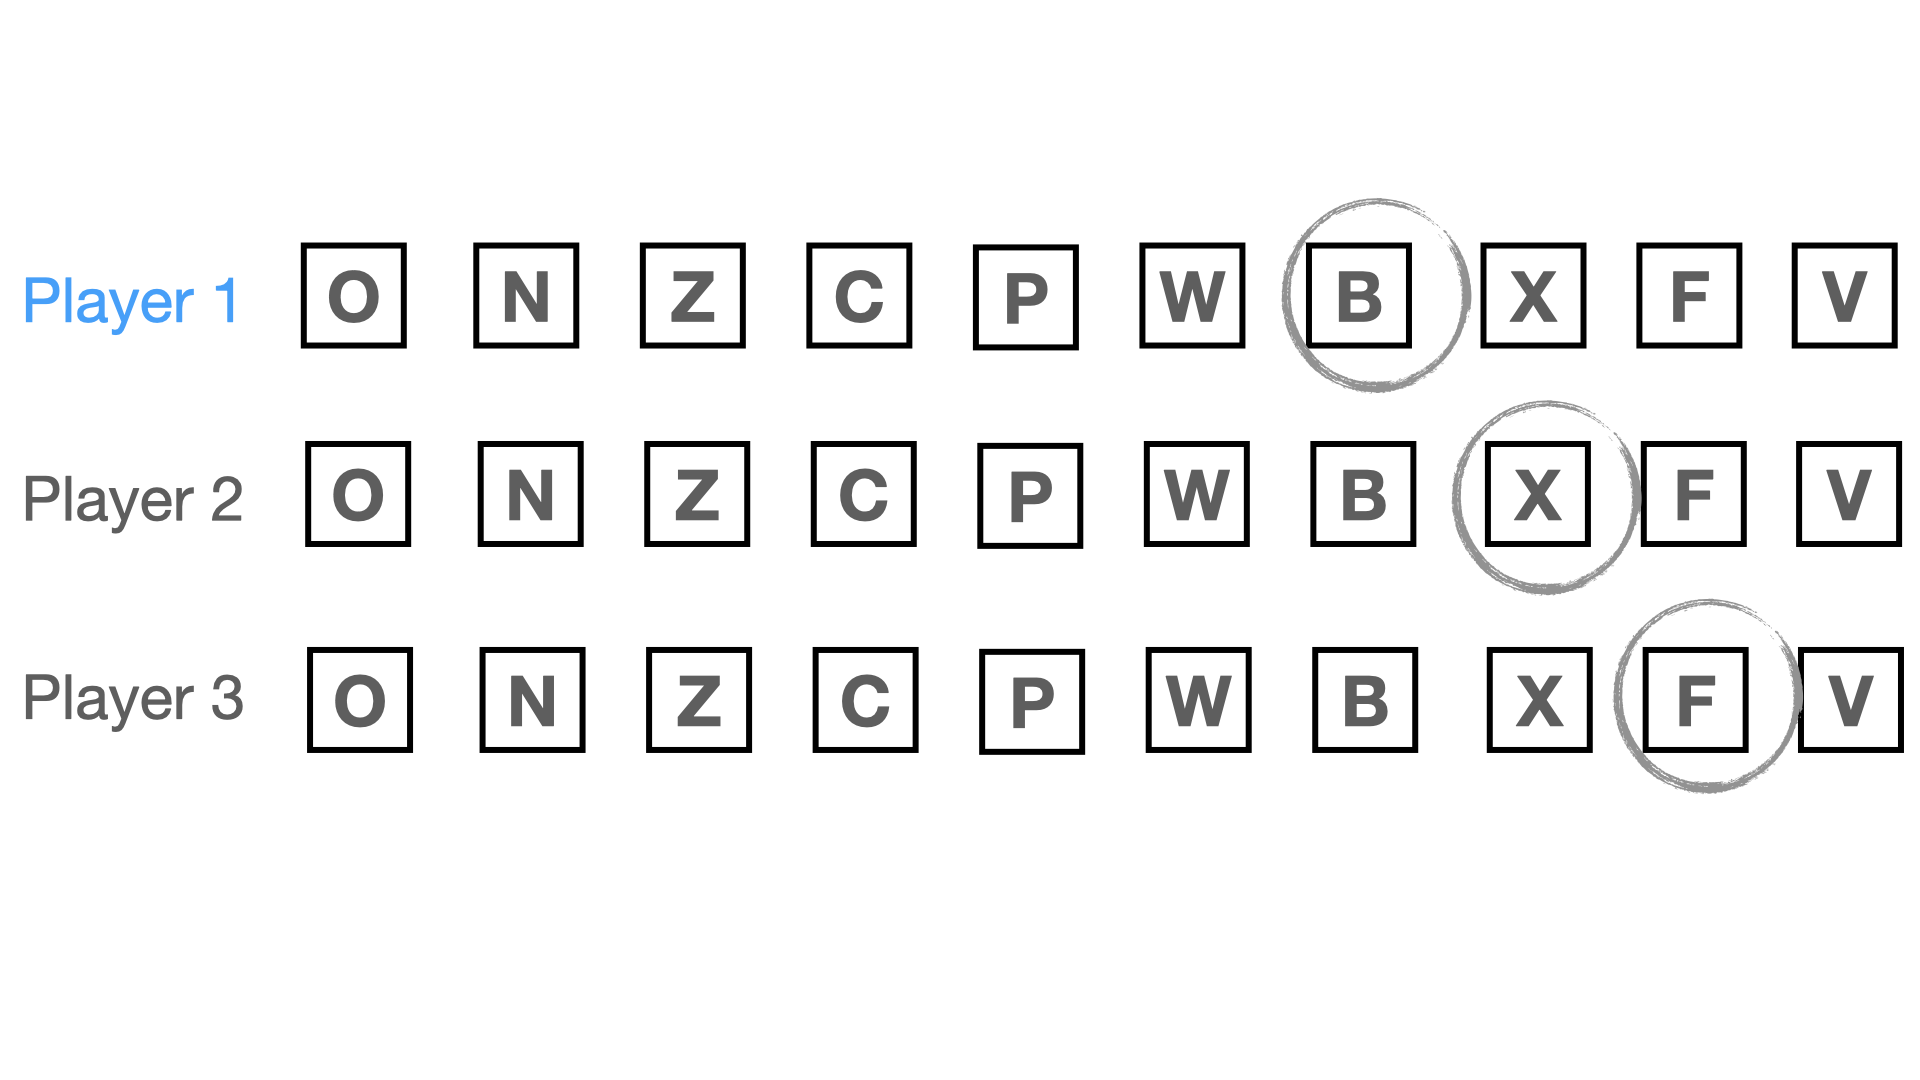
\includegraphics[width=0.6\textwidth,height=\textheight]{figures/stimuli/divergence_10_a.png}
&
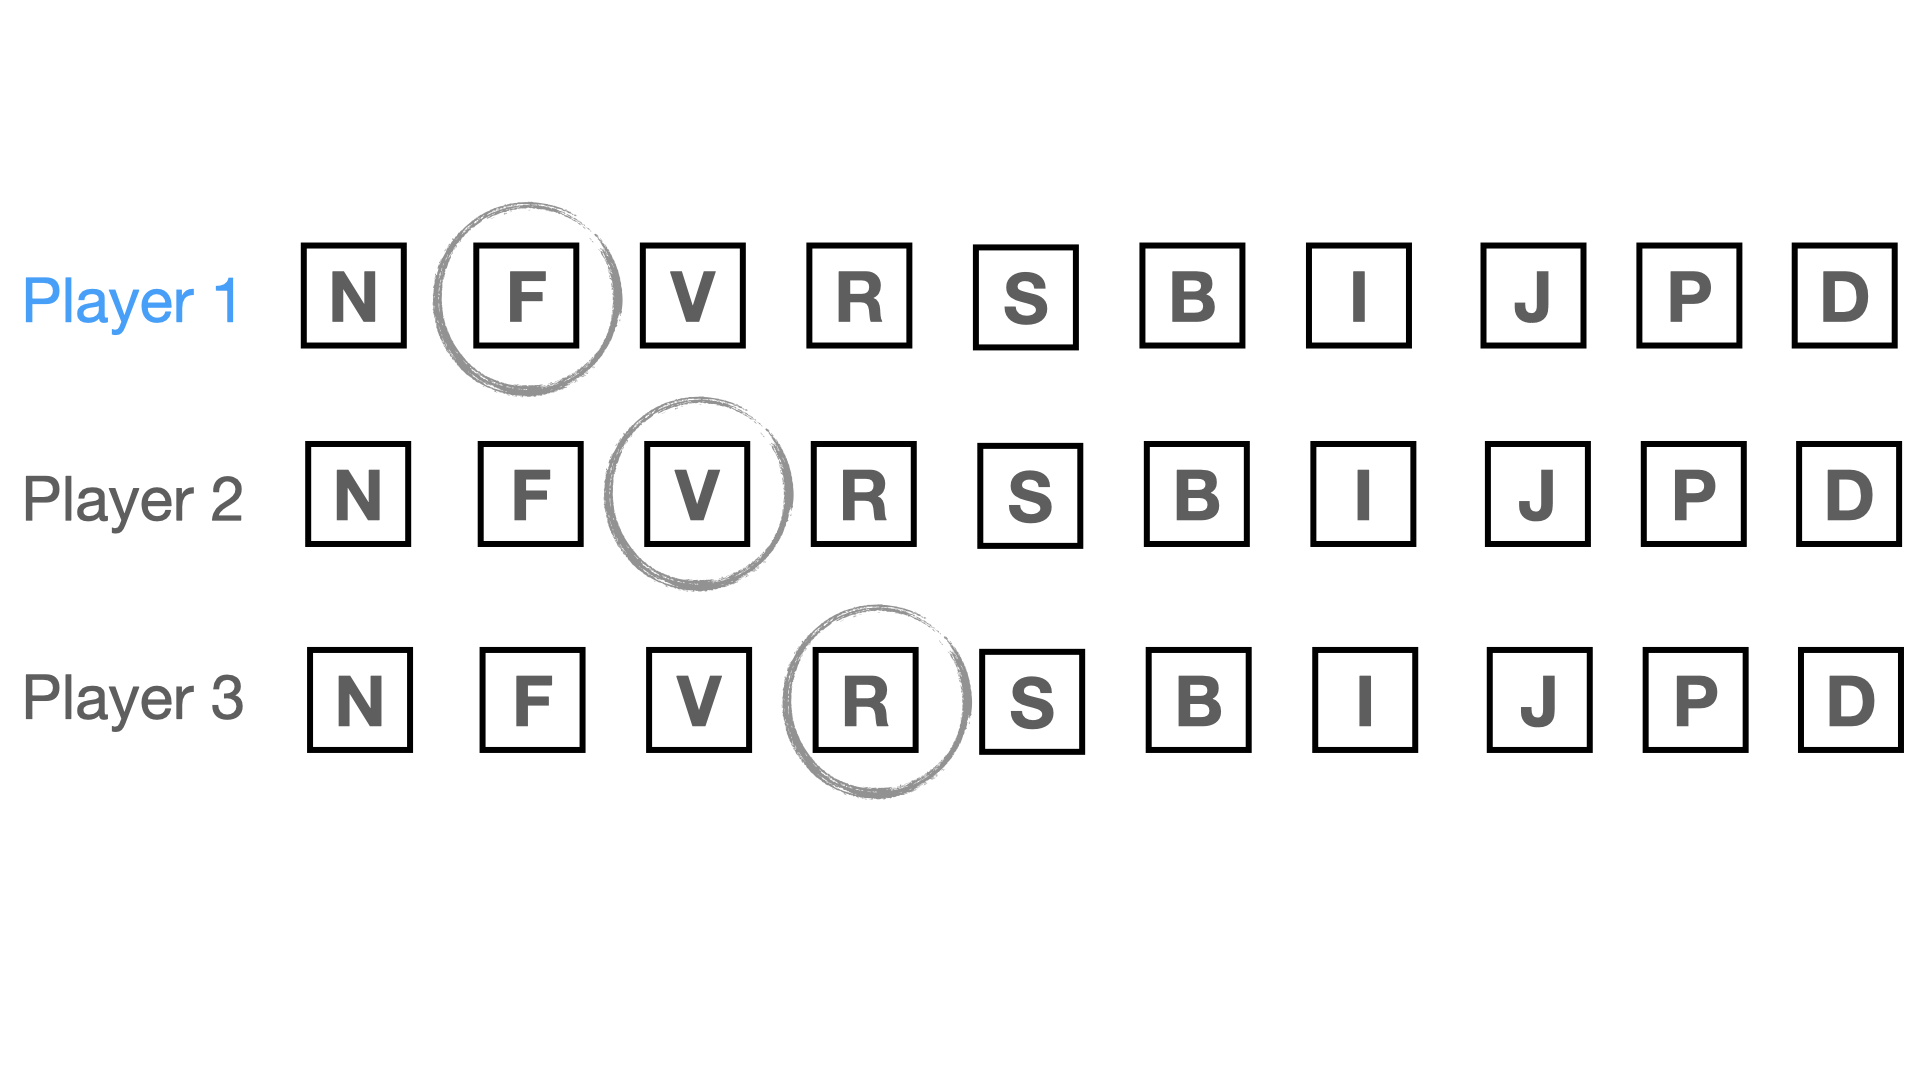
\includegraphics[width=0.6\textwidth,height=\textheight]{figures/stimuli/divergence_10_b.png} \\
majority (2) &
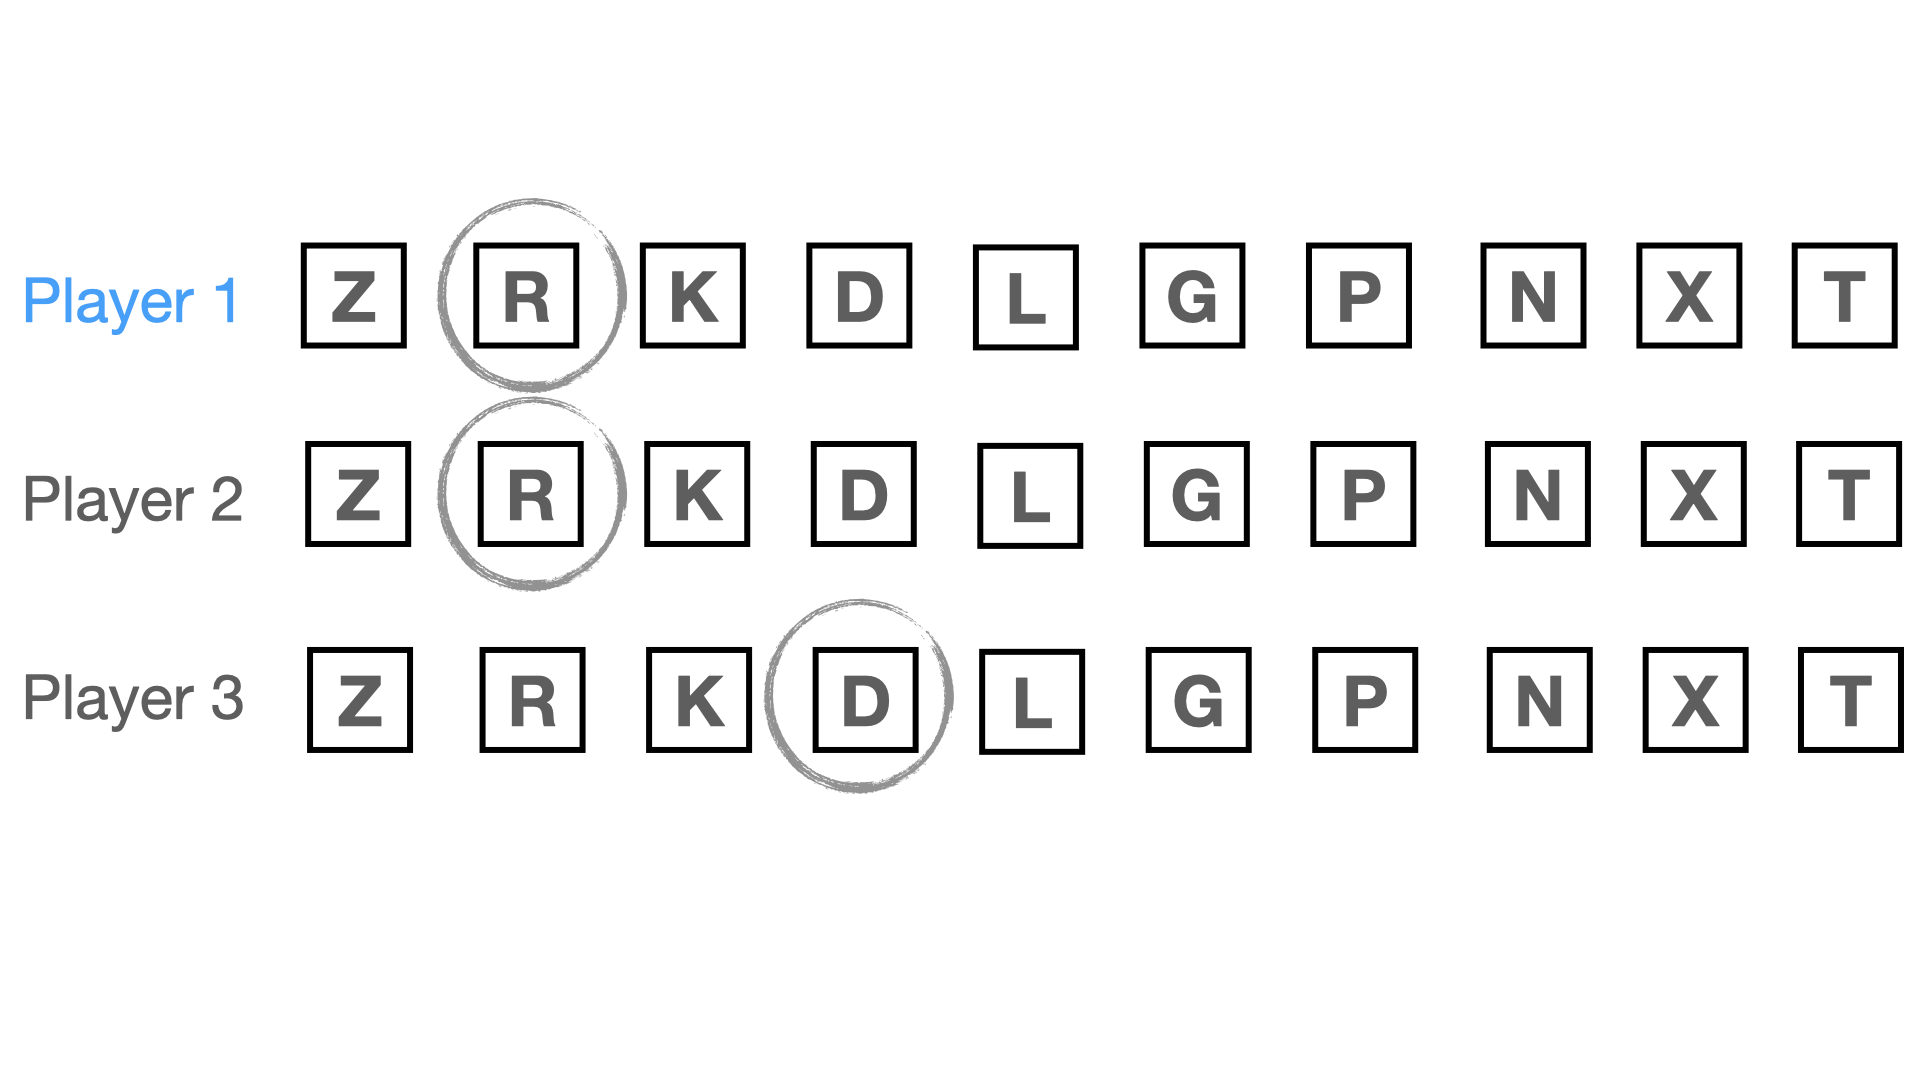
\includegraphics[width=0.6\textwidth,height=\textheight]{figures/stimuli/majority_10_a.png}
&
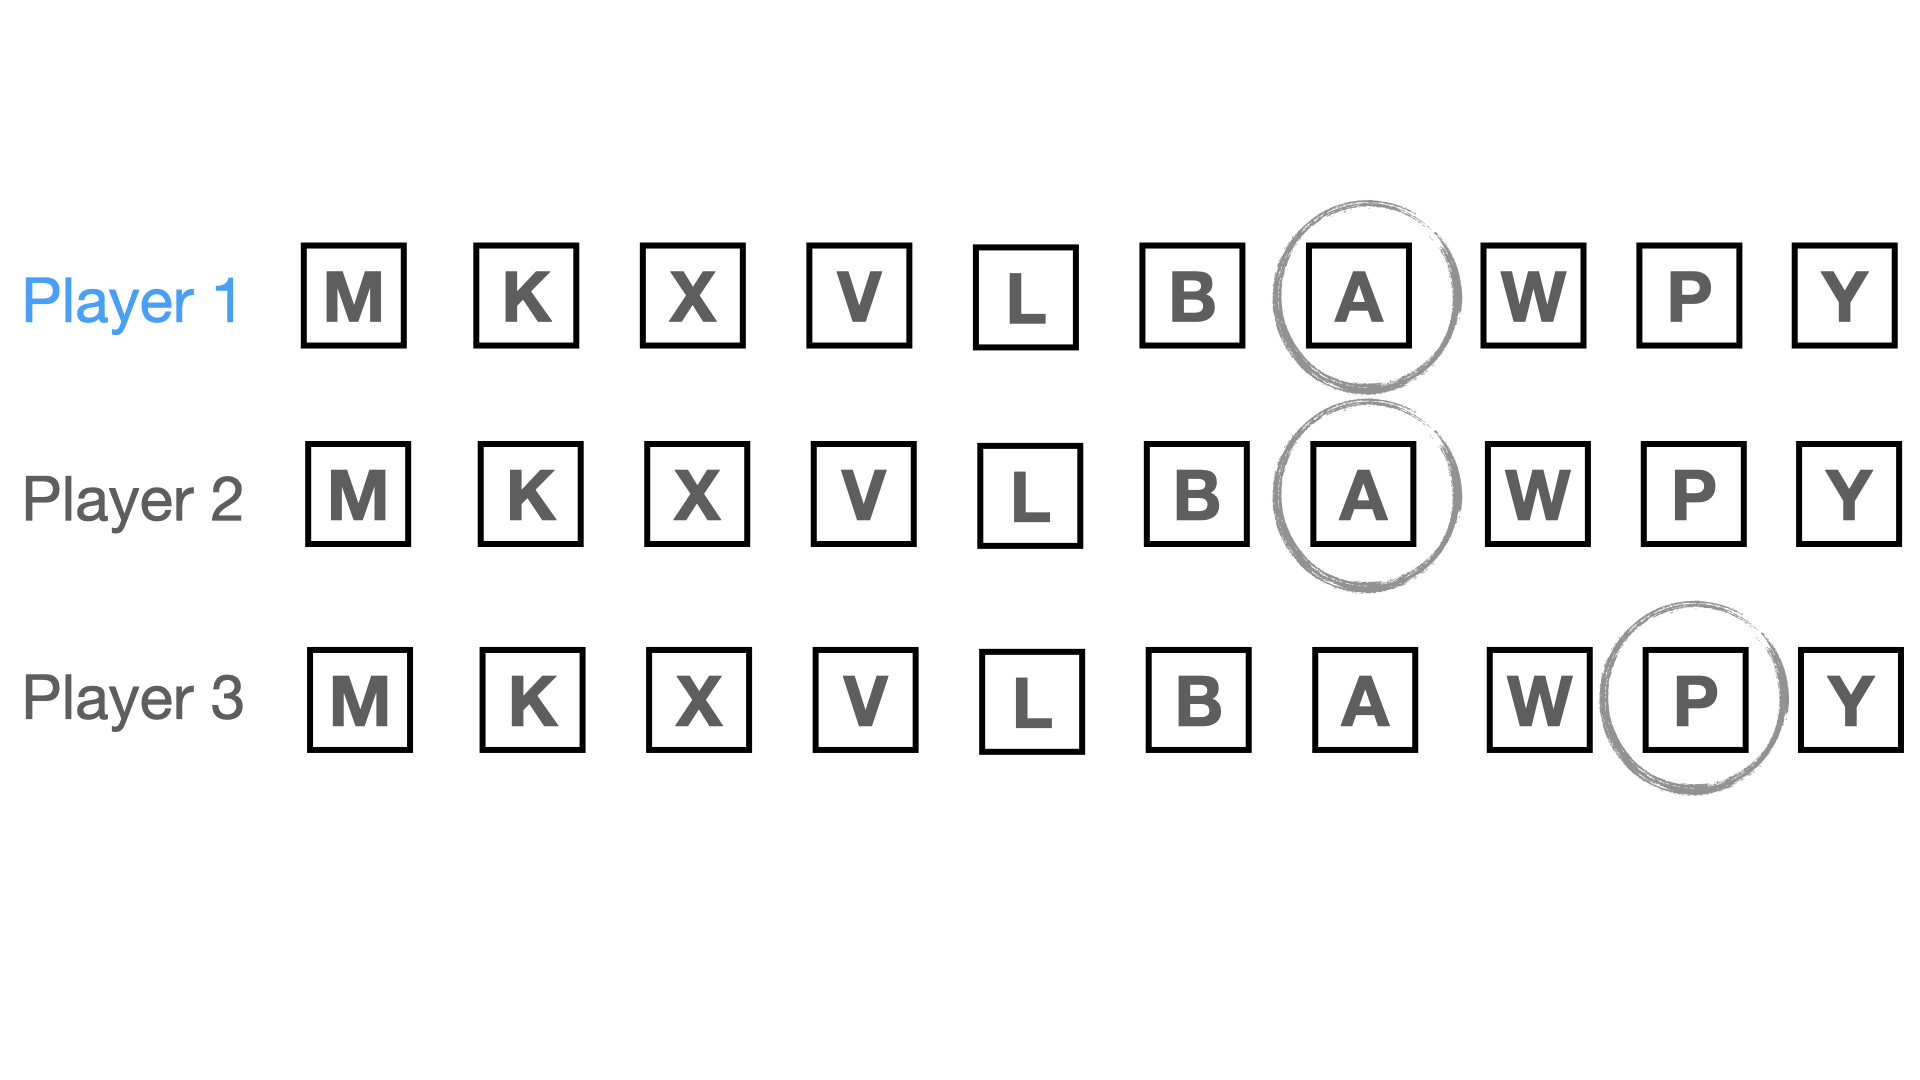
\includegraphics[width=0.6\textwidth,height=\textheight]{figures/stimuli/majority_10_b.png} \\
consensus (10) &
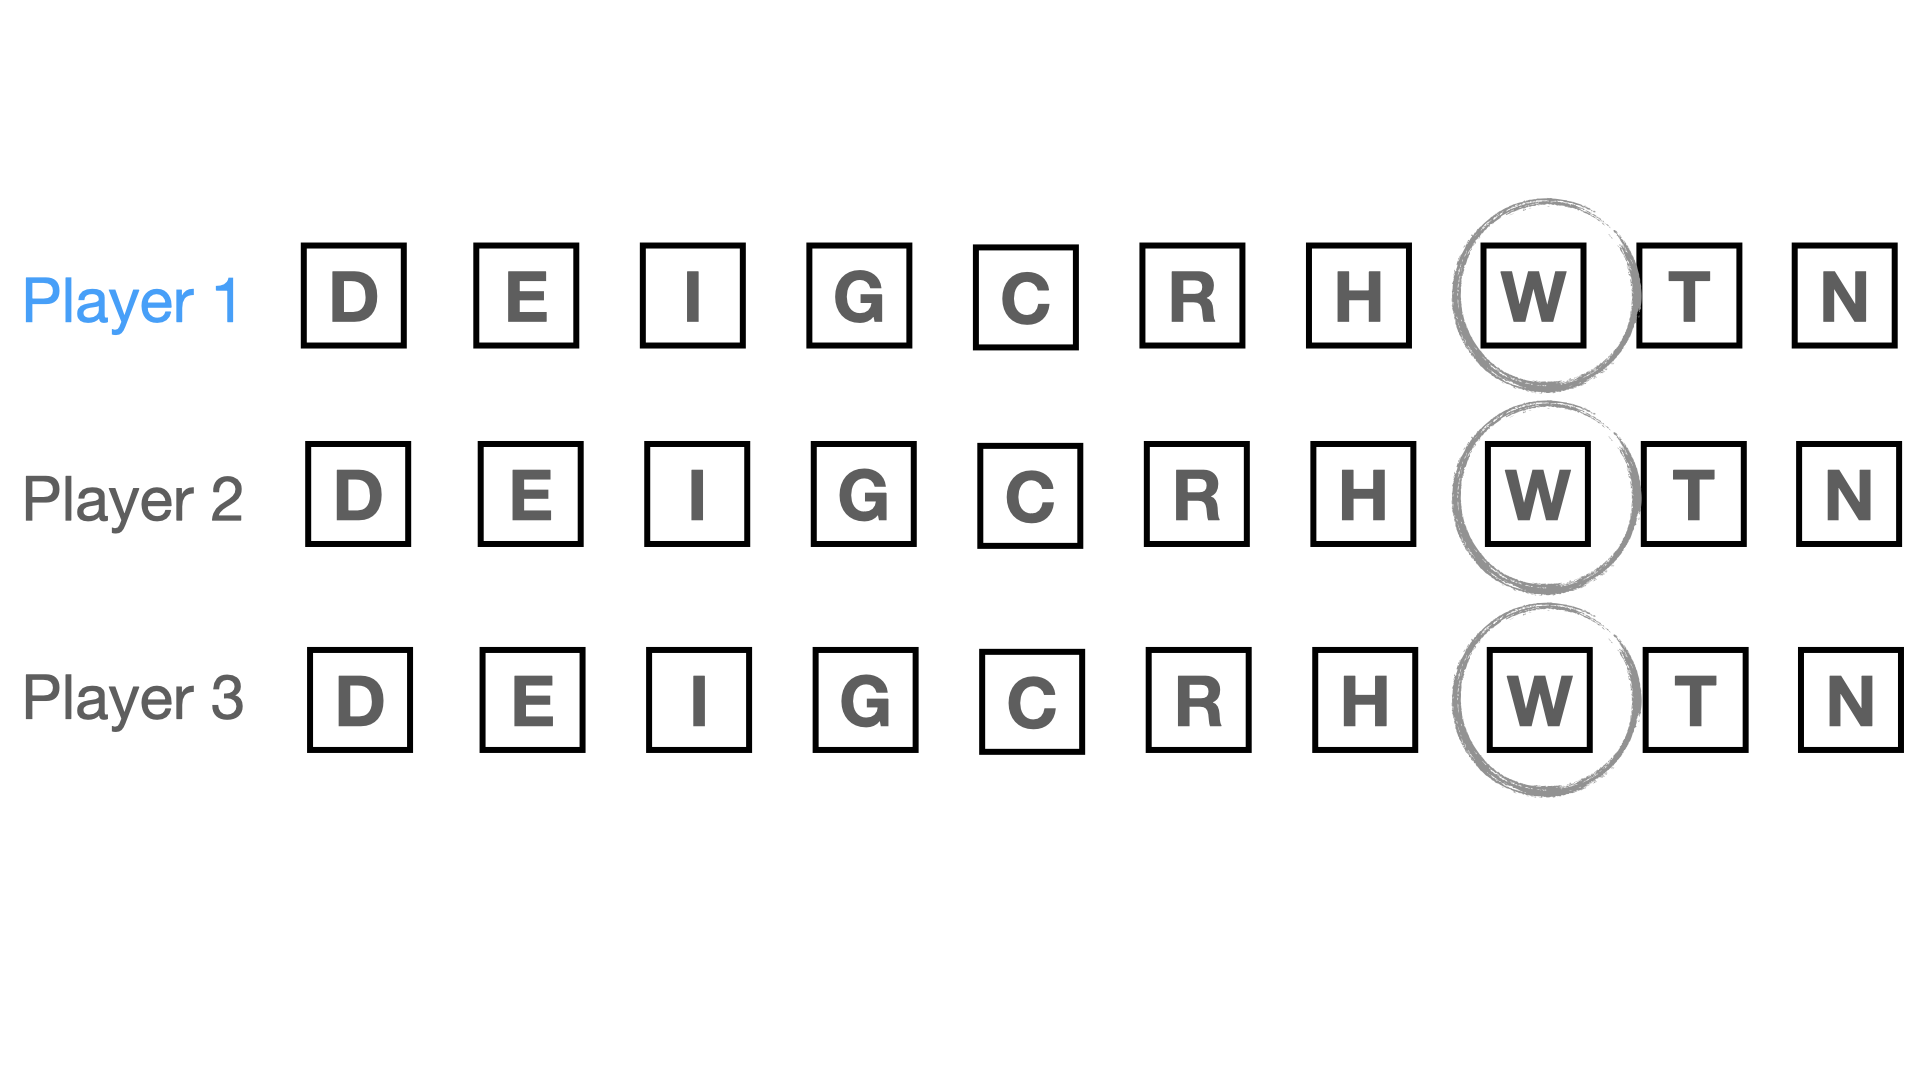
\includegraphics[width=0.6\textwidth,height=\textheight]{figures/stimuli/consensus_10_a.png}
&
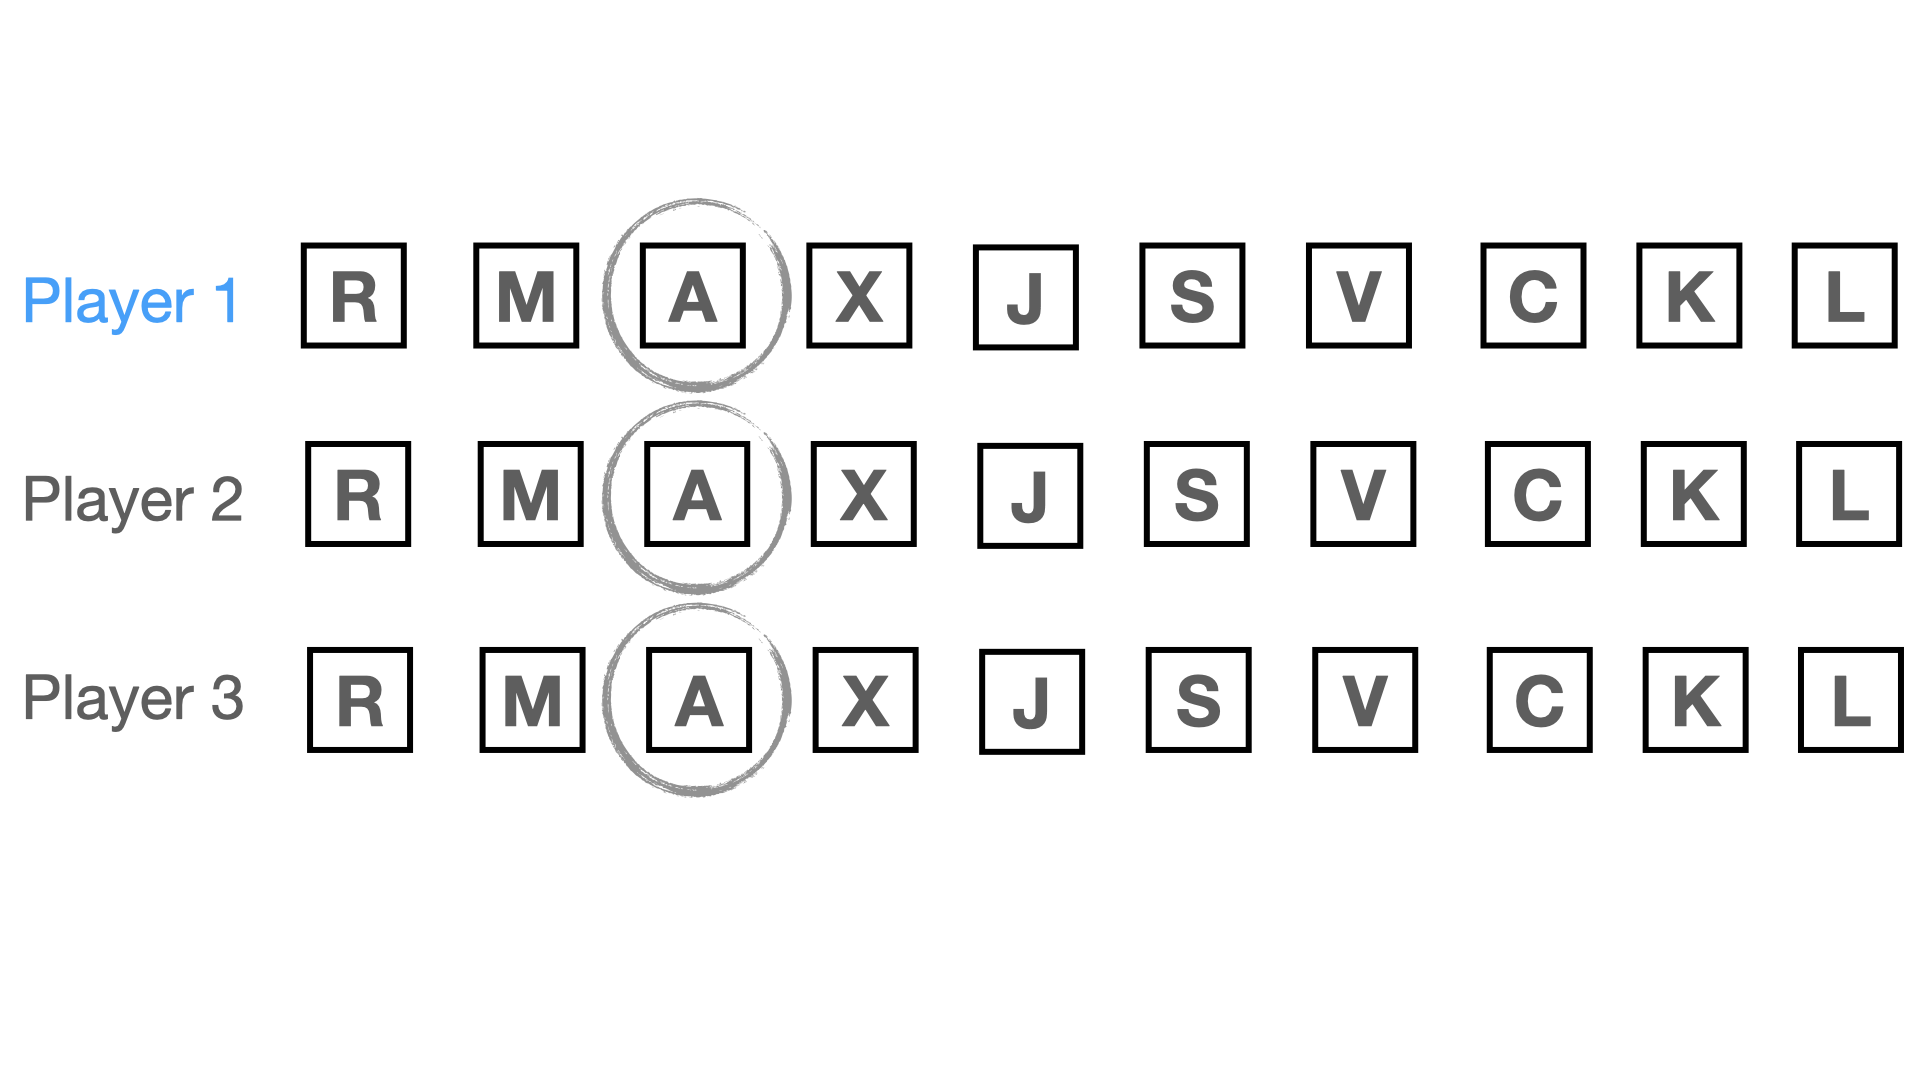
\includegraphics[width=0.6\textwidth,height=\textheight]{figures/stimuli/consensus_10_b.png} \\
\bottomrule()
\end{longtable}

\begin{longtable}[]{@{}
  >{\centering\arraybackslash}p{(\columnwidth - 4\tabcolsep) * \real{0.1608}}
  >{\centering\arraybackslash}p{(\columnwidth - 4\tabcolsep) * \real{0.4196}}
  >{\centering\arraybackslash}p{(\columnwidth - 4\tabcolsep) * \real{0.4196}}@{}}
\caption{Alternative stimuli for 3 options condition by levels of
convergence}\tabularnewline
\toprule()
\begin{minipage}[b]{\linewidth}\centering
Level
\end{minipage} & \begin{minipage}[b]{\linewidth}\centering
Version a)
\end{minipage} & \begin{minipage}[b]{\linewidth}\centering
Version b)
\end{minipage} \\
\midrule()
\endfirsthead
\toprule()
\begin{minipage}[b]{\linewidth}\centering
Level
\end{minipage} & \begin{minipage}[b]{\linewidth}\centering
Version a)
\end{minipage} & \begin{minipage}[b]{\linewidth}\centering
Version b)
\end{minipage} \\
\midrule()
\endhead
opposing majority (0) &
\includegraphics[width=0.6\textwidth,height=\textheight]{figures/stimuli/opp_majority_3_a_alt.png}
&
\includegraphics[width=0.6\textwidth,height=\textheight]{figures/stimuli/opp_majority_3_b_alt.png} \\
dissensus (1) &
\includegraphics[width=0.6\textwidth,height=\textheight]{figures/stimuli/divergence_3_a_alt.png}
&
\includegraphics[width=0.6\textwidth,height=\textheight]{figures/stimuli/divergence_3_b_alt.png} \\
majority (2) &
\includegraphics[width=0.6\textwidth,height=\textheight]{figures/stimuli/majority_3_a_alt.png}
&
\includegraphics[width=0.6\textwidth,height=\textheight]{figures/stimuli/majority_3_b_alt.png} \\
consensus (3) &
\includegraphics[width=0.6\textwidth,height=\textheight]{figures/stimuli/consensus_3_a_alt.png}
&
\includegraphics[width=0.6\textwidth,height=\textheight]{figures/stimuli/consensus_3_b_alt.png} \\
\bottomrule()
\end{longtable}

\begin{longtable}[]{@{}
  >{\centering\arraybackslash}p{(\columnwidth - 4\tabcolsep) * \real{0.1586}}
  >{\centering\arraybackslash}p{(\columnwidth - 4\tabcolsep) * \real{0.4207}}
  >{\centering\arraybackslash}p{(\columnwidth - 4\tabcolsep) * \real{0.4207}}@{}}
\caption{Alternative stimuli for 10 options condition by levels of
convergence}\tabularnewline
\toprule()
\begin{minipage}[b]{\linewidth}\centering
Level
\end{minipage} & \begin{minipage}[b]{\linewidth}\centering
Version a)
\end{minipage} & \begin{minipage}[b]{\linewidth}\centering
Version b)
\end{minipage} \\
\midrule()
\endfirsthead
\toprule()
\begin{minipage}[b]{\linewidth}\centering
Level
\end{minipage} & \begin{minipage}[b]{\linewidth}\centering
Version a)
\end{minipage} & \begin{minipage}[b]{\linewidth}\centering
Version b)
\end{minipage} \\
\midrule()
\endhead
opposing majority (0) &
\includegraphics[width=0.6\textwidth,height=\textheight]{figures/stimuli/opp_majority_10_a_alt.png}
&
\includegraphics[width=0.6\textwidth,height=\textheight]{figures/stimuli/opp_majority_10_b_alt.png} \\
dissensus (1) &
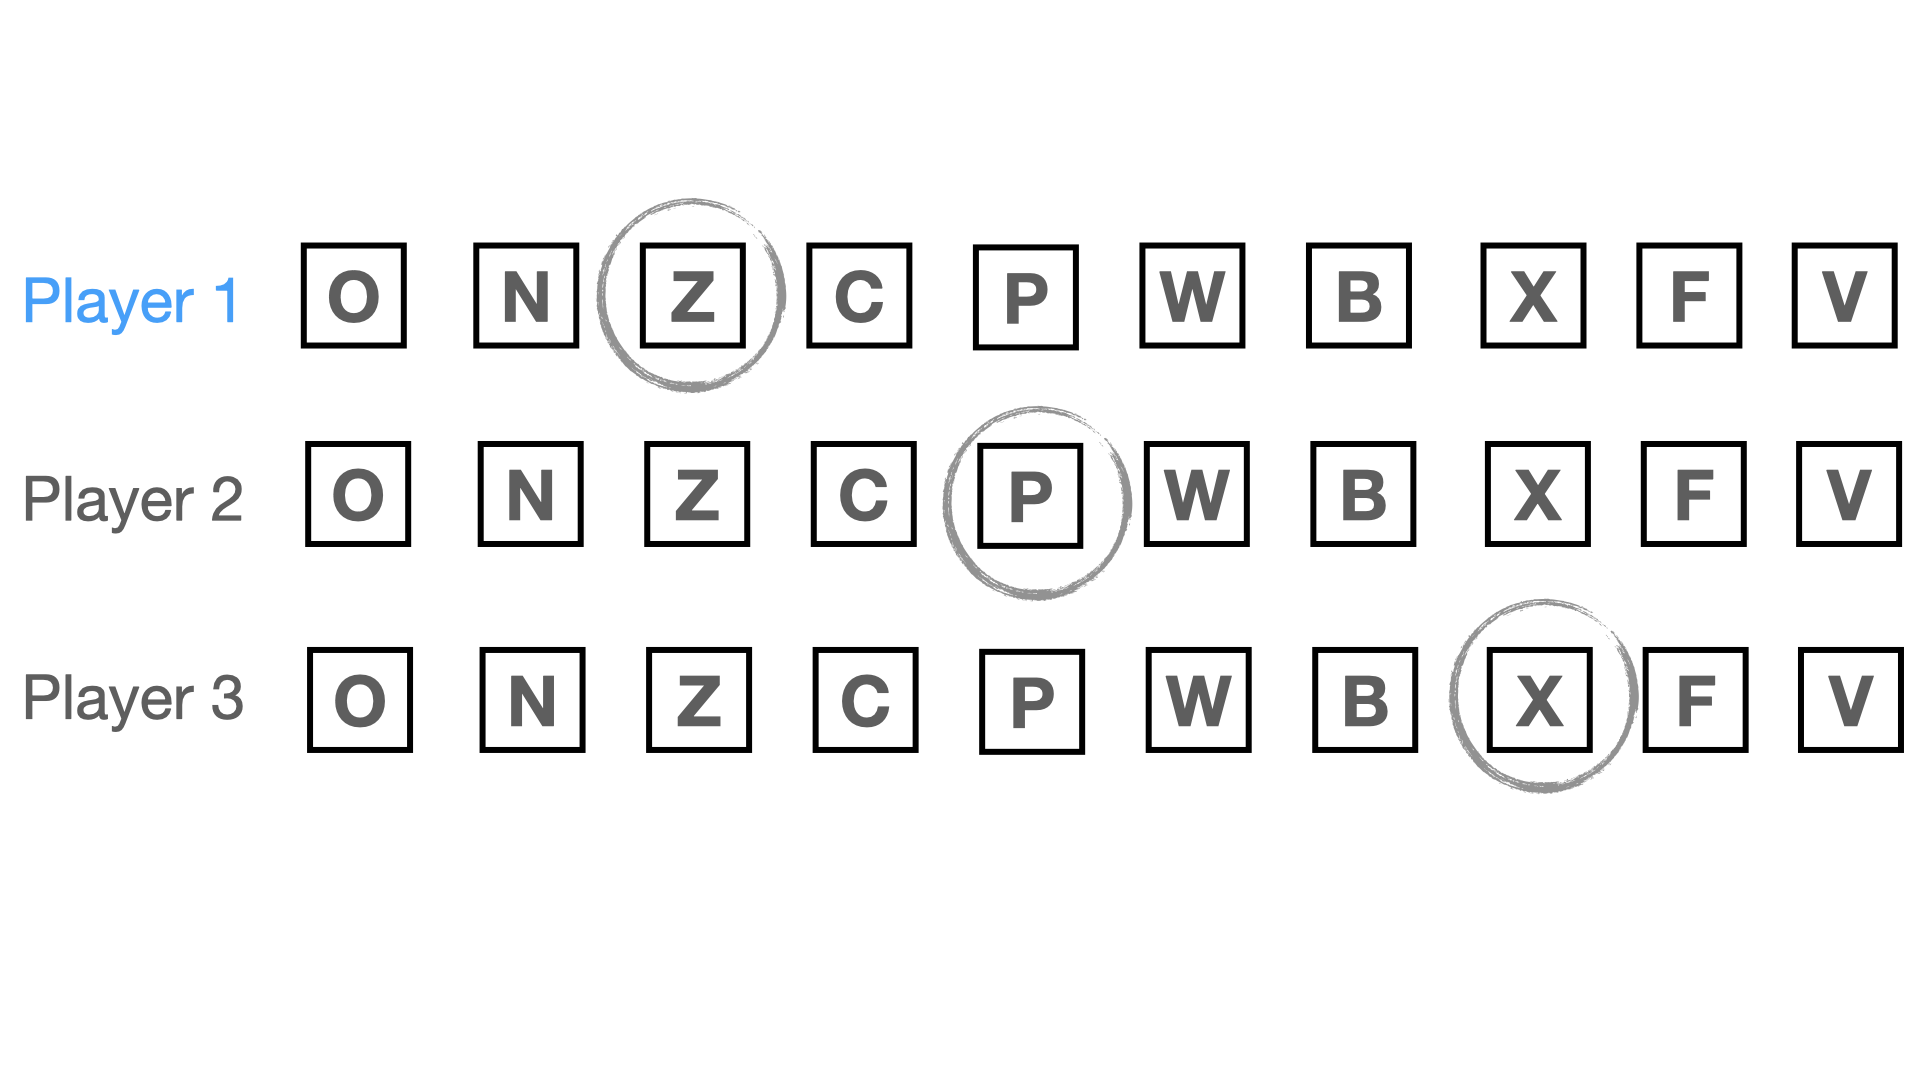
\includegraphics[width=0.6\textwidth,height=\textheight]{figures/stimuli/divergence_10_a_alt.png}
&
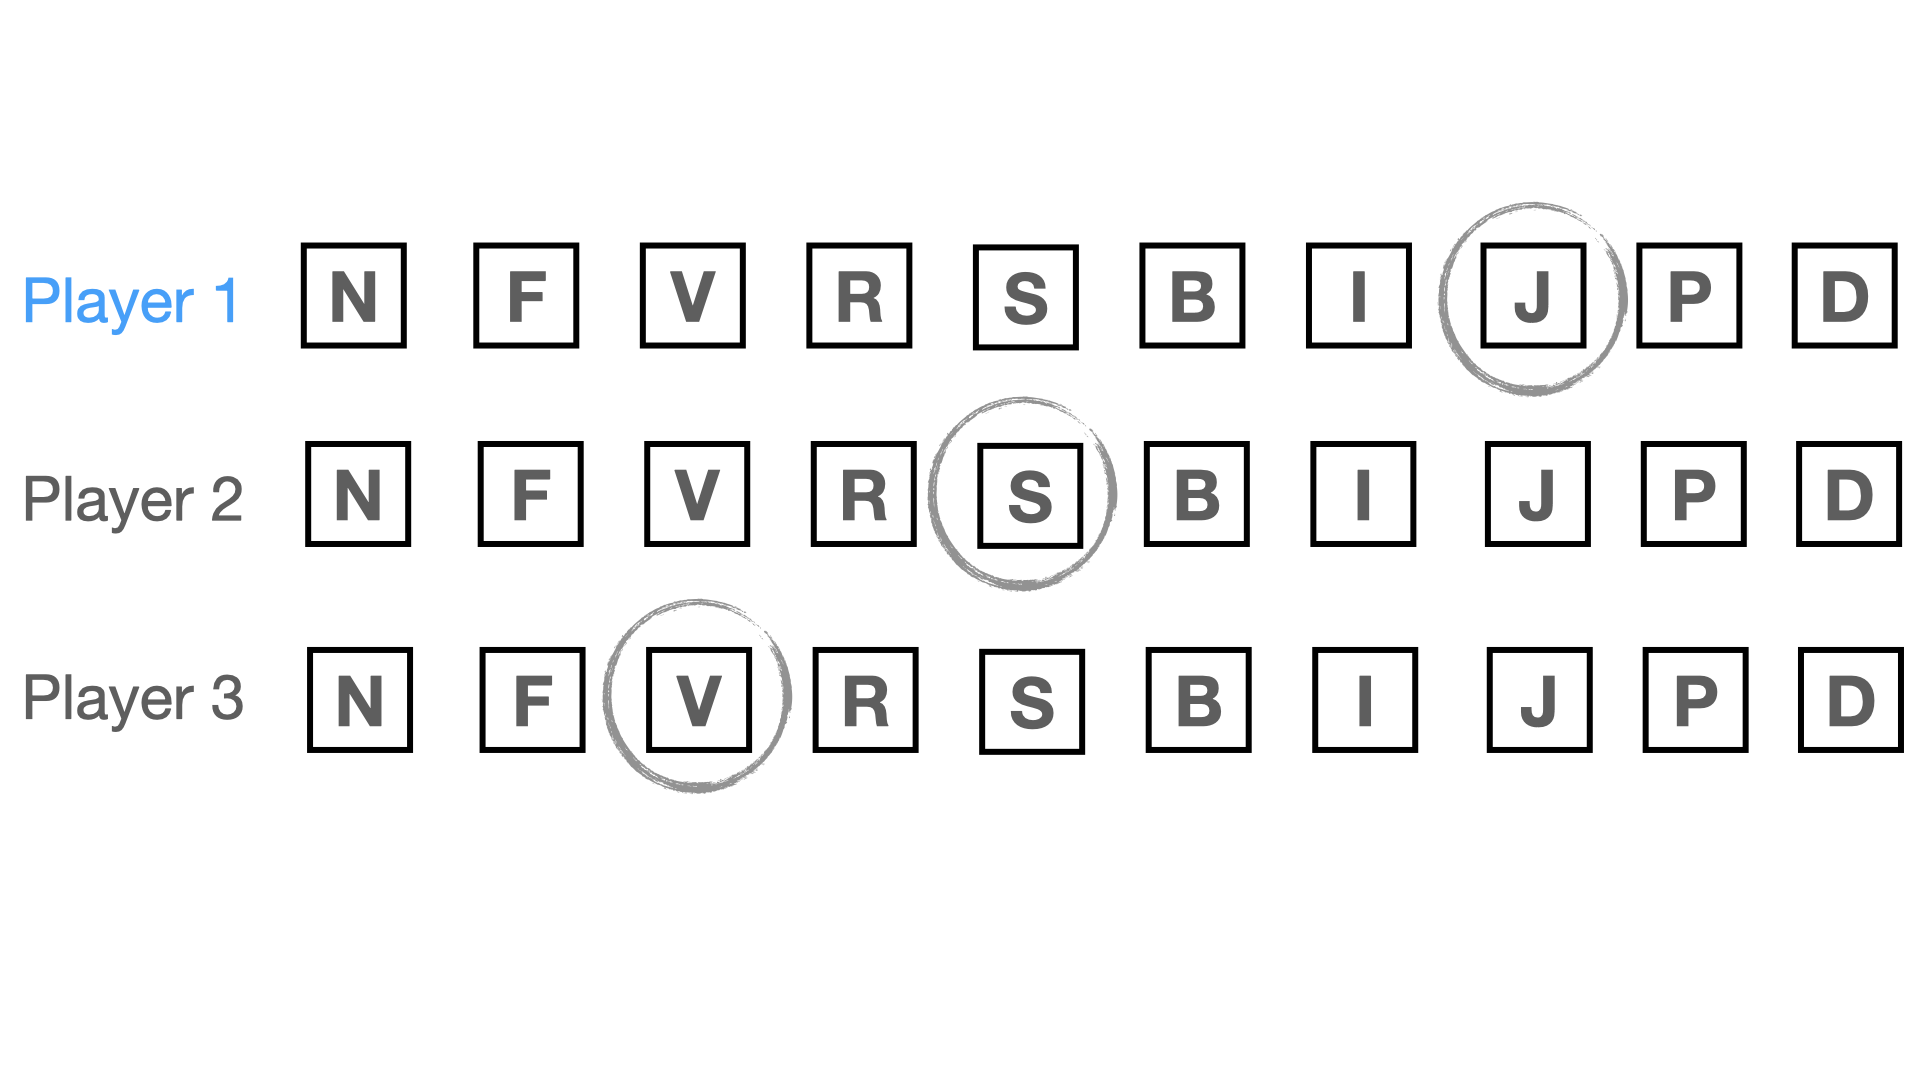
\includegraphics[width=0.6\textwidth,height=\textheight]{figures/stimuli/divergence_10_b_alt.png} \\
majority (2) &
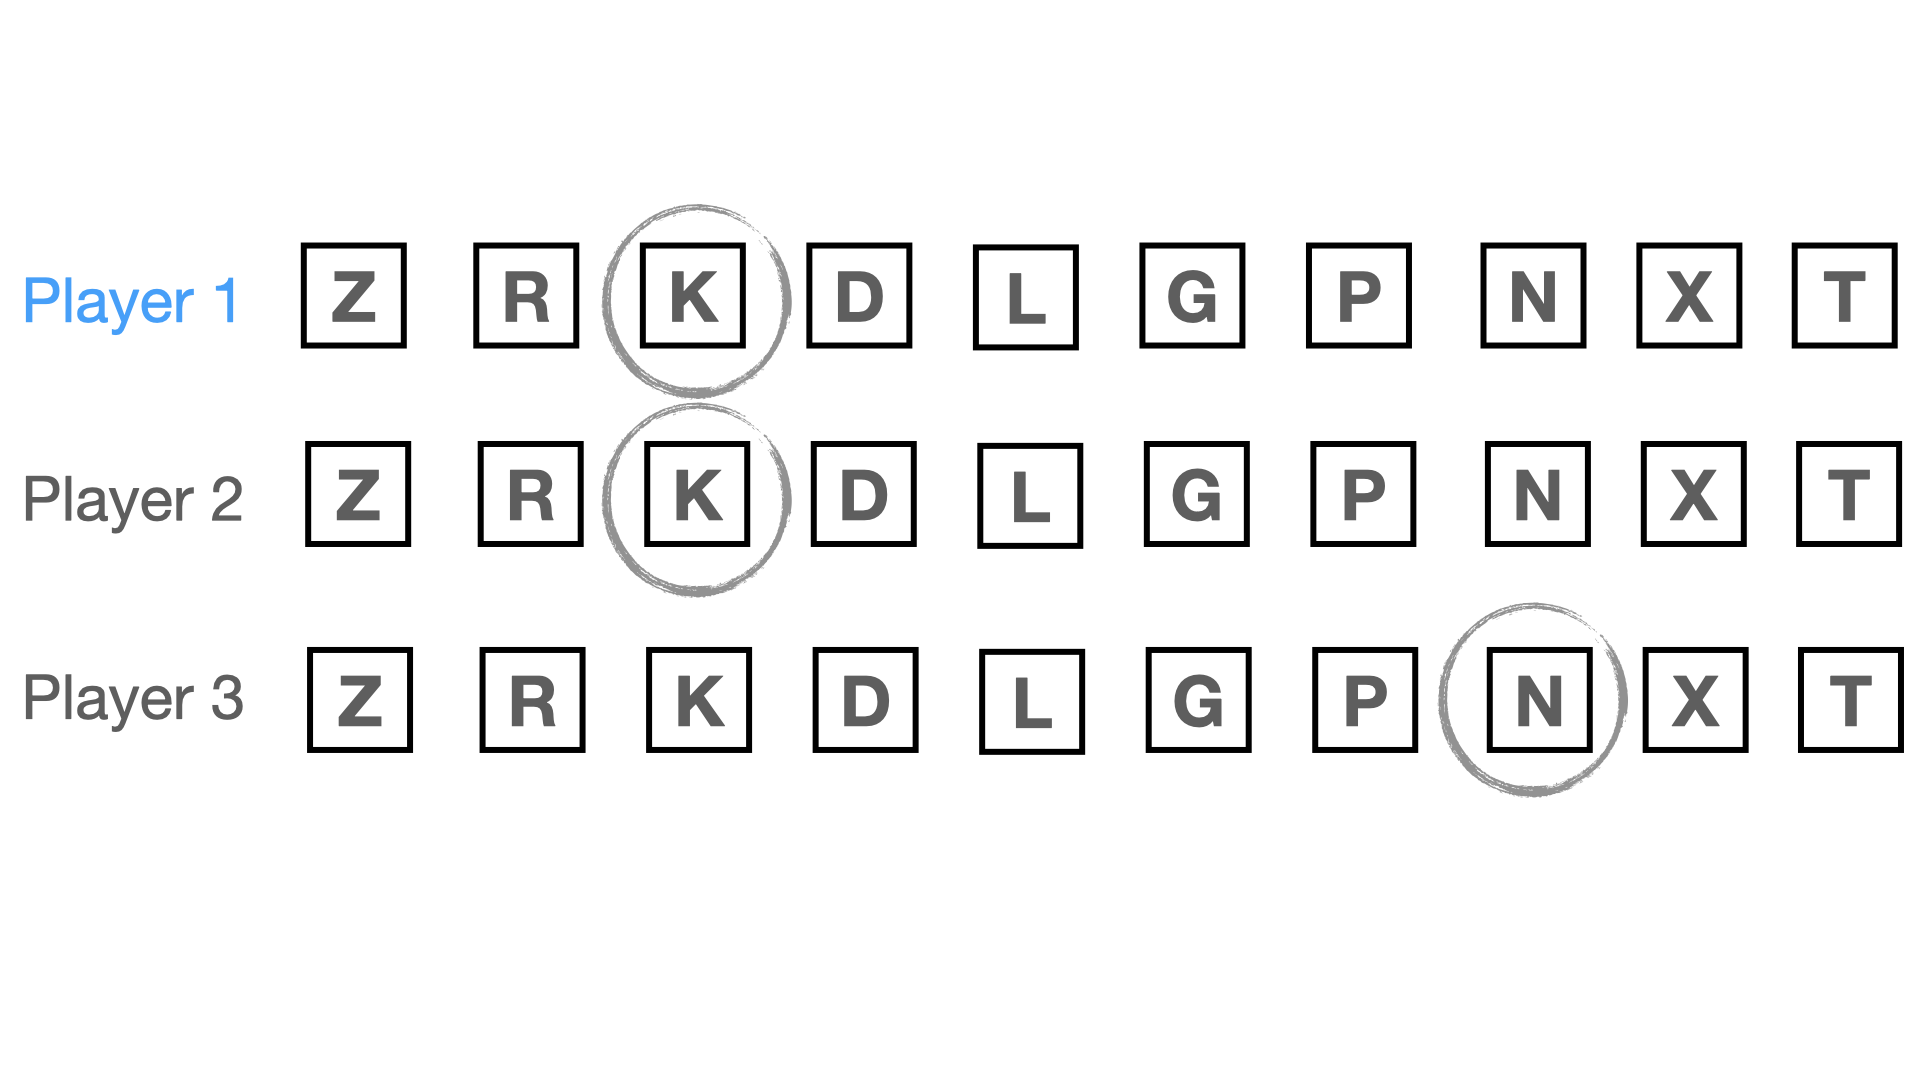
\includegraphics[width=0.6\textwidth,height=\textheight]{figures/stimuli/majority_10_a_alt.png}
&
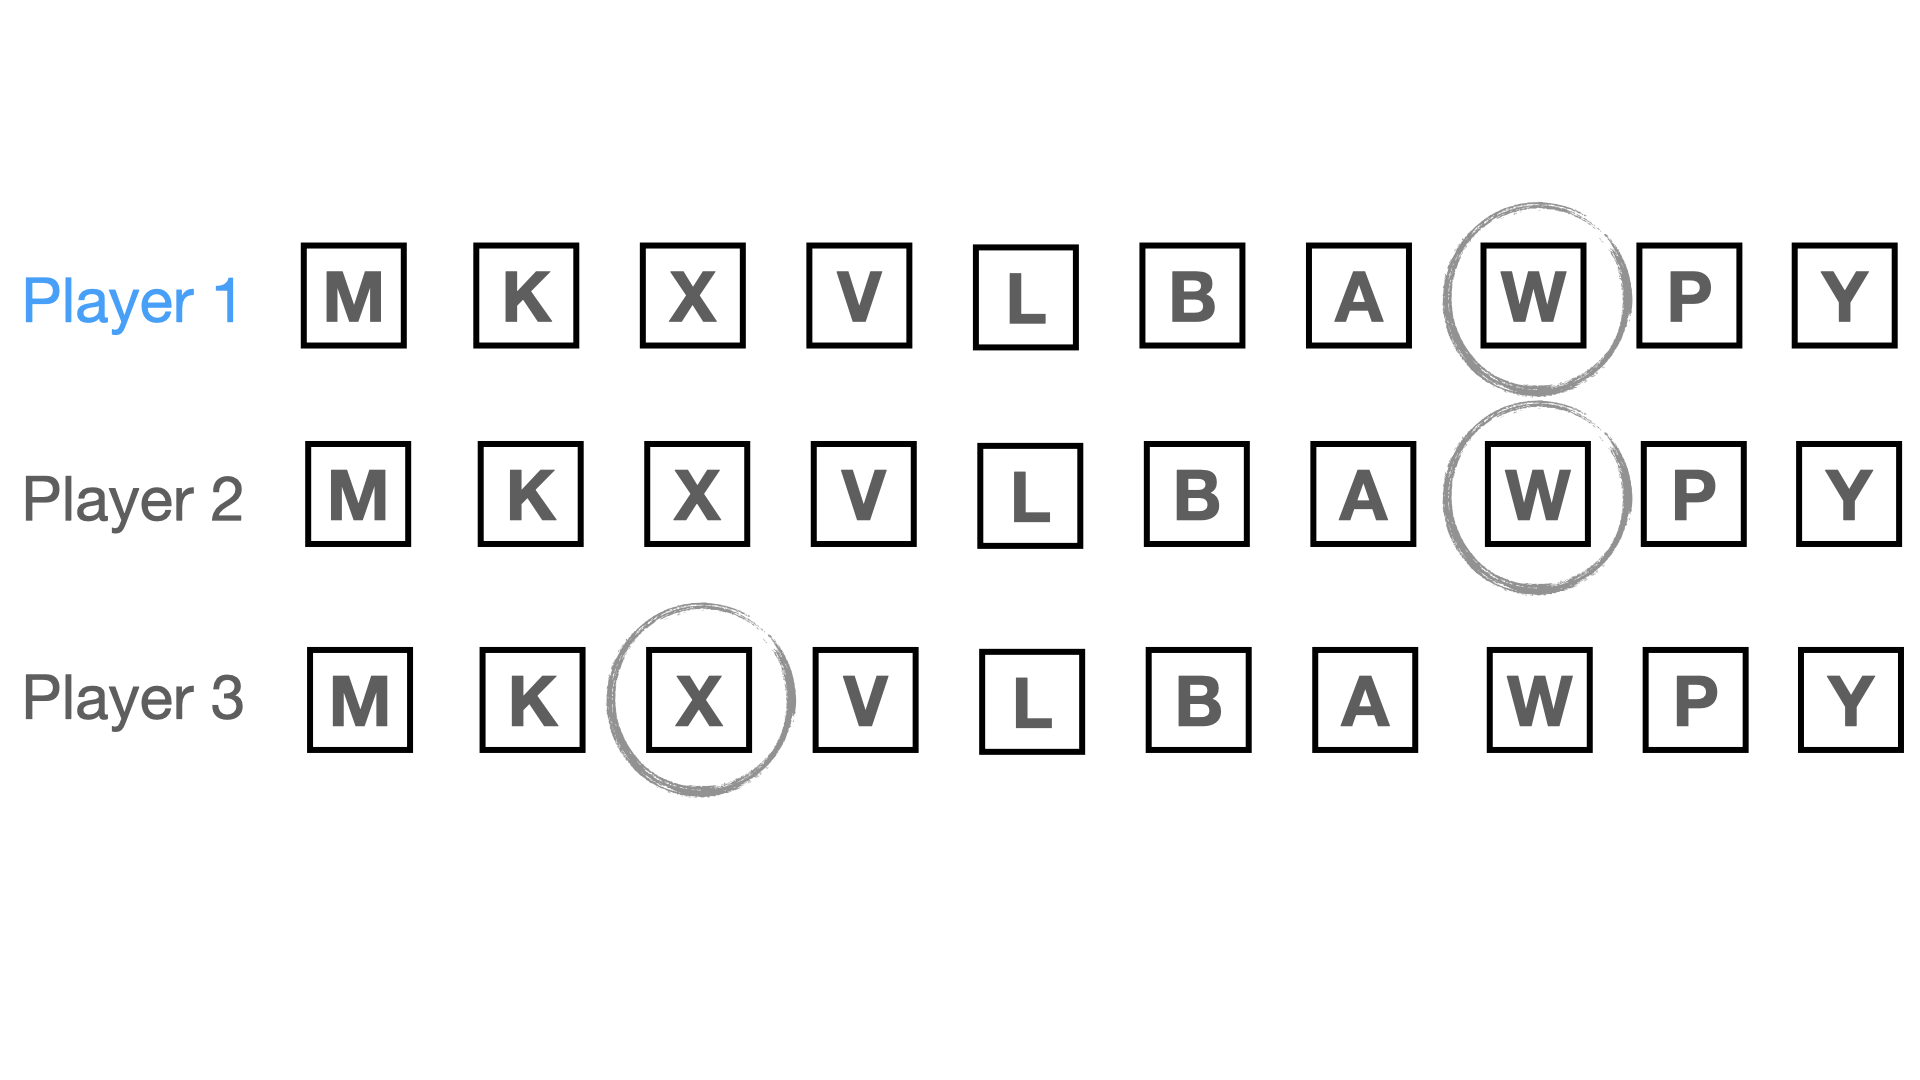
\includegraphics[width=0.6\textwidth,height=\textheight]{figures/stimuli/majority_10_b_alt.png} \\
consensus (10) &
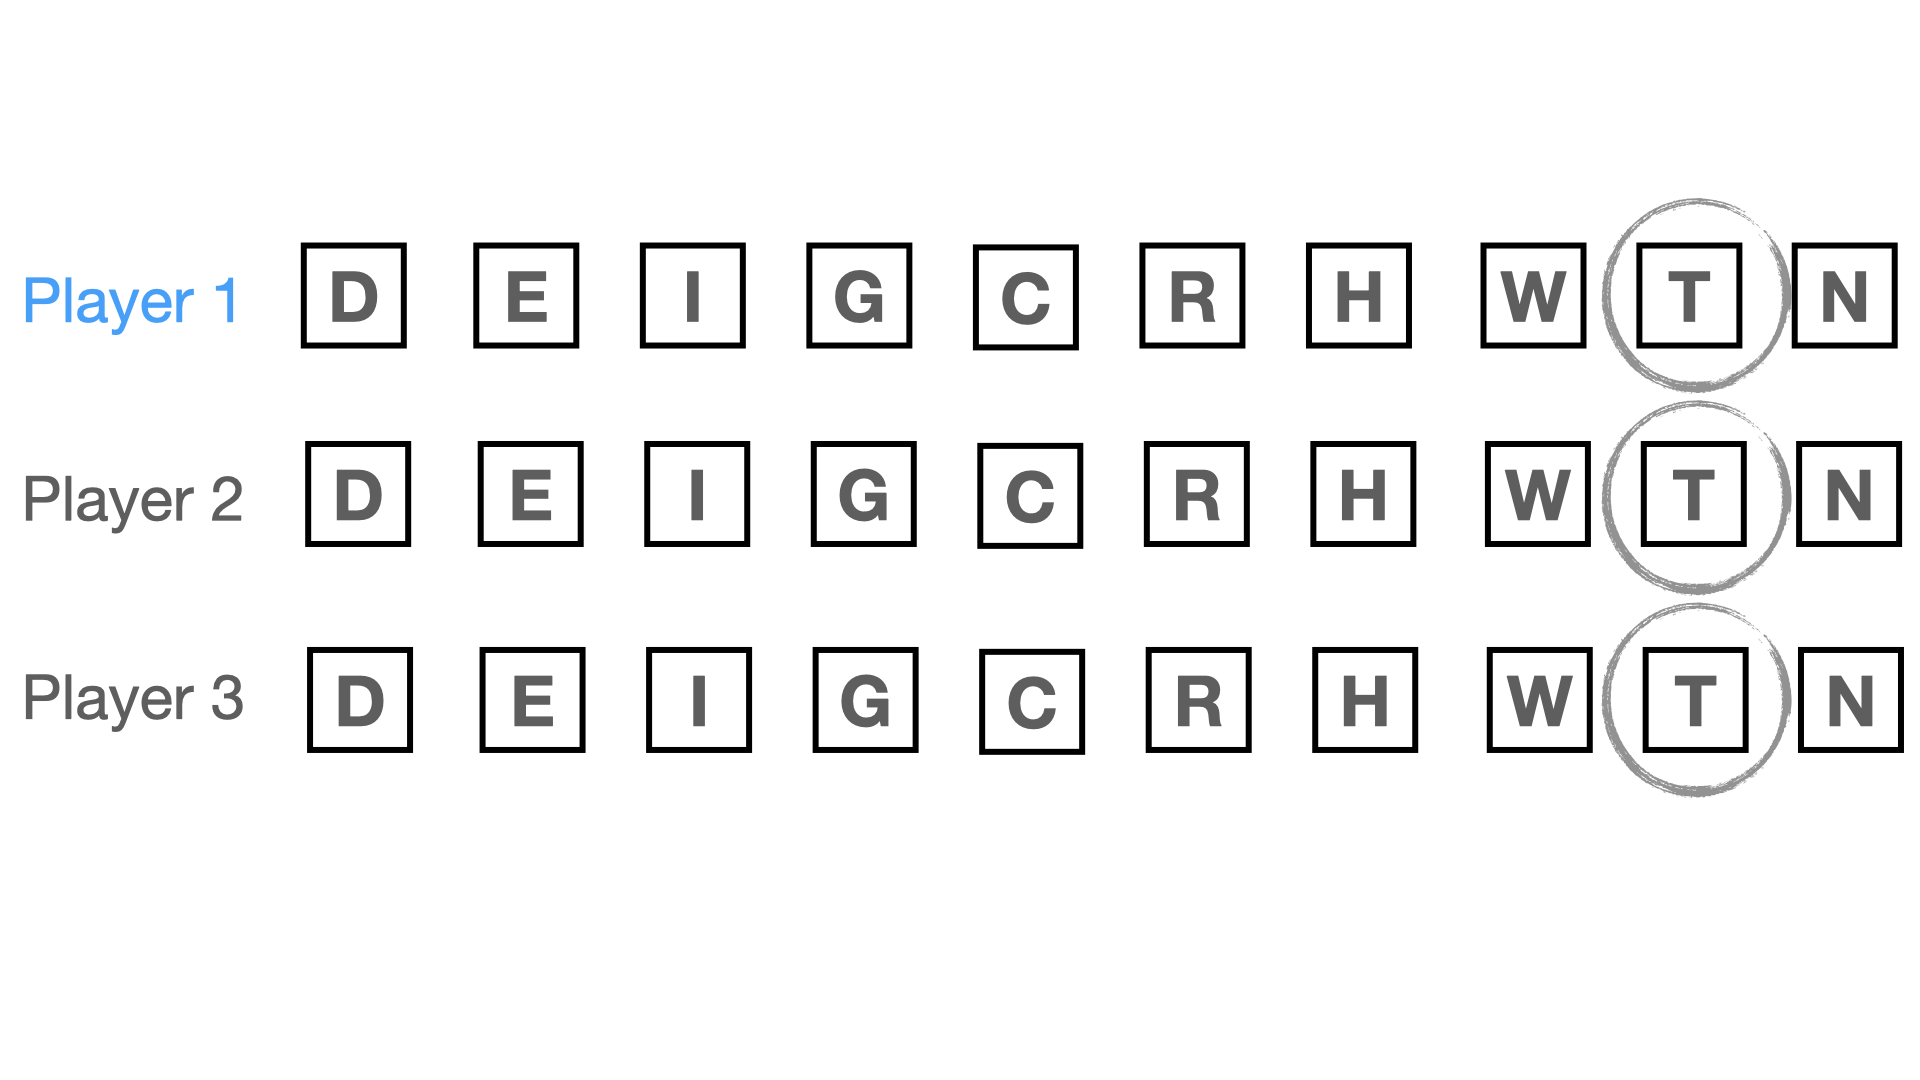
\includegraphics[width=0.6\textwidth,height=\textheight]{figures/stimuli/consensus_10_a_alt.png}
&
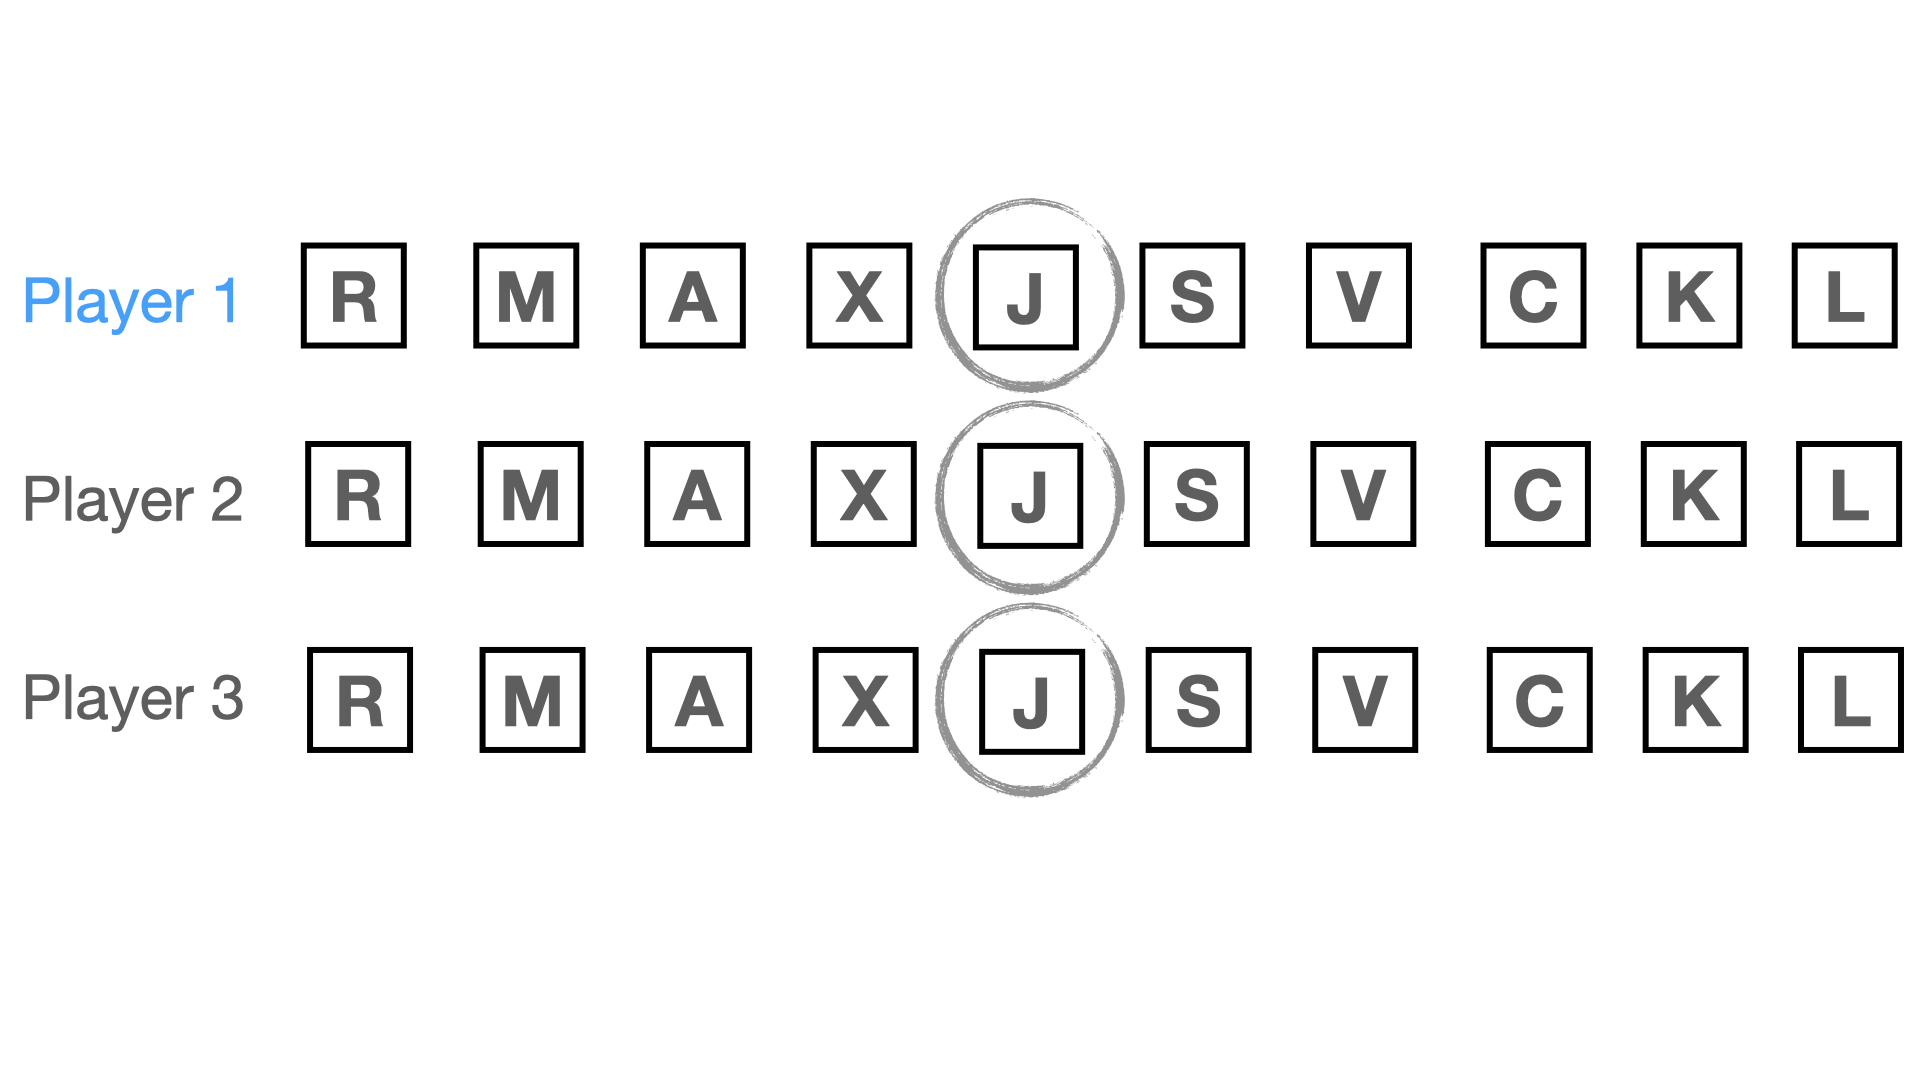
\includegraphics[width=0.6\textwidth,height=\textheight]{figures/stimuli/consensus_10_b_alt.png} \\
\bottomrule()
\end{longtable}

\end{document}
